% Options for packages loaded elsewhere
\PassOptionsToPackage{unicode}{hyperref}
\PassOptionsToPackage{hyphens}{url}
% !TeX program = pdfLaTeX
\documentclass[12pt]{article}
\usepackage{amsmath}
\usepackage{graphicx,psfrag,epsf}
\usepackage{enumerate}
\usepackage[]{natbib}
\usepackage{textcomp}


%\pdfminorversion=4
% NOTE: To produce blinded version, replace "0" with "1" below.
\newcommand{\blind}{0}

% DON'T change margins - should be 1 inch all around.
\addtolength{\oddsidemargin}{-.5in}%
\addtolength{\evensidemargin}{-1in}%
\addtolength{\textwidth}{1in}%
\addtolength{\textheight}{1.7in}%
\addtolength{\topmargin}{-1in}%

%% load any required packages here



% tightlist command for lists without linebreak
\providecommand{\tightlist}{%
  \setlength{\itemsep}{0pt}\setlength{\parskip}{0pt}}

% From pandoc table feature
\usepackage{longtable,booktabs,array}
\usepackage{calc} % for calculating minipage widths
% Correct order of tables after \paragraph or \subparagraph
\usepackage{etoolbox}
\makeatletter
\patchcmd\longtable{\par}{\if@noskipsec\mbox{}\fi\par}{}{}
\makeatother
% Allow footnotes in longtable head/foot
\IfFileExists{footnotehyper.sty}{\usepackage{footnotehyper}}{\usepackage{footnote}}
\makesavenoteenv{longtable}



\IfFileExists{bookmark.sty}{\usepackage{bookmark}}{\usepackage{hyperref}}
\IfFileExists{xurl.sty}{\usepackage{xurl}}{} % add URL line breaks if available
\hypersetup{
  pdftitle={(working title) Control mechanisms for working with consultants},
  hidelinks,
  pdfcreator={LaTeX via pandoc}}



\begin{document}


\def\spacingset#1{\renewcommand{\baselinestretch}%
{#1}\small\normalsize} \spacingset{1}


%%%%%%%%%%%%%%%%%%%%%%%%%%%%%%%%%%%%%%%%%%%%%%%%%%%%%%%%%%%%%%%%%%%%%%%%%%%%%%

\if0\blind
{
  \title{\bf (working title) Control mechanisms for working with
consultants}

  \author{
        Roel Peters \\
    Antwerp Management School\\
      }
  \maketitle
} \fi

\if1\blind
{
  \bigskip
  \bigskip
  \bigskip
  \begin{center}
    {\LARGE\bf (working title) Control mechanisms for working with
consultants}
  \end{center}
  \medskip
} \fi

\bigskip

\noindent%
 

\vfill

\newpage
\spacingset{1.9} % DON'T change the spacing!

\section{Introduction}\label{introduction}

\section{Defining ``Digital
Consultancy''}\label{defining-digital-consultancy}

``Digital consultancy'' is defined as consultancy in (either or both)
technological and organizational aspects of digital transformation. The
following two sections substantiate this definition by elaborating on
the two concepts that comprise this definition. First, six properties
that define ``consultancy'' are discussed, followed by an elaboration on
``digital transformation.''

\subsection{Consultancy}\label{consultancy}

Consultants, or management consultants, have been described through a
multitude of metaphors and nicknames: ``capitalism's commissars''
\citep[ 93]{thrift2005}, ``shadowy figures operating in the background
but exercising considerable influence'' \citep[ 31]{kipping2012},
``agents of a modern rationalistic and universalistic culture'' \citep[
190]{kipping2012}, ``institutionally approved agents'' \citep[
193]{kipping2012}, ``marketized experts'' \citep[ 265]{furusten2012},
``magical figures, shamans or witch doctors'' \citep[ 68]{fincham2002},
``puppet masters'' \citep[ 69]{fincham2002}, ``knowledge entrepreneurs
that promote emotionally charged, enthusiastic, and unreasoned
discourse'' \citep[ 37]{leicht2006}, ``supra-experts'' \citep[
94]{kieser2006}, ``improvising experts'' \citep[ 272]{furusten2009},
``brochuremanship'' \citep[ 75]{levine1982} and simply ``The Big Con''
\citep{mazzucato2023}.

Their work makes use of a vague body of knowledge described as
``elusive'', ``fuzzy'', ``perishable'', ``indeterminate'', ``esoteric'',
``fluid'' and ``changeable'' \citep{muzio2011}. Consequently, for buyers
it is hard to know what they need and what they get, and for sellers of
consultancy it is hard to know what to offer \citep[ 266]{furusten2012}.
Furthermore, consultancy is marked by very low professionalization since
occupational entry is unprotected, the supply of labor is unregulated
and there is no formal accreditation. \citep[ 20]{fincham2006}
Practicing ``consultancy'' is the main criterion of membership with
competences and ``time spent in the industry'' as the main
differentiators.

These remarks are prima facie evidence that no consensus around the
definition exists, and what they do is extremely hard to describe.
\citet[24]{kipping2012} states that ``definitions of management
consultancy are problematic because the permeable boundaries of the
industry have resulted in significant shifts over time in the
composition of the industry. This means that what comprises consulting
work is dynamic, ever shifting, and contested as new firms enter the
industry and techniques deemed formerly appropriate, change. Although
the industry is characterized by periodic structural shifts, at its
heart it is an advisory activity built on the client--consultant
relationship. {[}\ldots{]} it is perhaps this chimeral ability to avoid
precise definition and to be able to constantly reinvent its core
services to meet ever changing understandings of the problems that beset
contemporary organizations, which partly underpins its growing economic
importance.''

The following definition of ``consultancy'' is used throughout this
paper.

\begin{quote}
\emph{Consultancy is a service offered by an external service provider.
Although the responsibilities of a consultant are highly contingent on
the client organization and consultancy can take many forms and require
a variety of expertise, its goal is to establish change in the
procedures, organizational structure or tools of a client organization.
Finally, the success of a consultancy engagement is often determined by
the interactivity between a consultancy firm and the client
organization.}
\end{quote}

The sections below unpack this definition and elaborate on the six
properties that it comprises.

\subsubsection{External}\label{external}

\citet[138]{chowdhury2021} describes consultants as ``external advisors
to corporations, nonprofits, governments, and any other forms of
organizations.''

\subsubsection{Change}\label{change}

Clearly, the construct of a ``consultant'' cannot be described by the
topic that they work on, nor their academic and professional background,
accreditation or membership. Instead, we should look at their goal(s):
\citet[1]{werr1986} implies that there is always a change process
between clients and consultants. This is confirmed by
\citet[12]{kipping2000} who states that ``management consultancies earn
money through changing current procedures in client organizations.''
Although this change is often described by consultants as a `tailored
solution', consultants provide a service, which is inherently intangible
(compared to the `solid' nature of products) and hard to evaluate
\citep[ 348]{fincham1999}, especially because an evaluation should not
only account for the content of the changes, but also in terms of the
competence development of the client, as a result of the change process
\citep[ 17]{werr1986}.

Although consultants' goal is to establish change in an organization,
their role is often symbolic. As external consultants, associated with
their ``quest for knowledge'' and their ``quest for excellence'', they
are \citep[ 9-13]{pellegrin2006} well-equipped for legitimizing hard
decisions, signaling importance and providing meaning.

Establishing change is what sets consultancy apart from temporary
staffing. ``A temp is generally not supposed to change the work
practices at the client organization. A consultant is often expected to
do just that, or at least to provide an alternative point of view.''
\citep[ 5]{furusten2000}

The aspect of change is also important for drawing boundaries between
consultancy and outsourcing. Consultants are often hired for defining a
problem and presenting a solution at the same time \citep[
272]{furusten2009}, while outsourcing simply delivers the solution. In
that sense, outsourcing is the practice of obtaining goods or services
from an external provider, as a substitute for sourcing it internally
\citep[ 2]{lacity2012}, for a contractually agreed monetary fee and
period of time \citep[ 20-21]{leimeister2010}. Or in the words of
\citet[374]{zhu2001}: ``the process of transferring the responsibility
for a specific business function from an employee group to a
non-employee group.'' While early IT outsourcing initiatives were rather
``total'' \citet{willcocks1995} in nature, outsourcing individual
business functions is now a more common activity \citep[ 377]{zhu2001},
and focus has shifted from cost saving to quality, productivity,
flexibility and technological diversity \citep[ 185]{kirilov2012}. This
implies that outsourcing, unlike consultancy, is not about changing a
procedure or service, but rather ensuring continuation, or
implementation, by a third-party provider\footnote{\emph{Prima facie},
  this could be interpreted as a departure from the work by
  \citet{loh1992} and \citet{venkatraman1994}, who claim that IT
  outsourcing is an ``administrative innovation, {[}\ldots{]} involving
  significant changes in the routines used by the organization to deal
  with its tasks of internal arrangements and external alignments.''
  However, while there is indeed a firm-level change \citep[
  14]{nelson1985}, in the sense of who is responsible for a specific
  (part of a) procedure, the procedure or service involved does not
  change \emph{an sich.}}.

Finally, \citet[272-273]{furusten2009} argues that consultants not only
act as agents of change, but often as agents of stability. Consultants
are often perceived as ``relatively stable by {[}\ldots{]} employees,
stakeholders and other external counterparts'', this ``builds confidence
for the organization. The more stable an organization is experienced as
being, the greater its ability to concentrate on its core activities.''

\subsubsection{Contingent}\label{contingent}

Being a consultant implies taking on a variety of responsibilities
throughout a certain time span. Although many consultants have
structured methodologies, which are converging across the industry
\citep[ 17]{werr1986}, ``{[}c{]}onsultants operate in an intense
environment that regularly entails new challenges.'' \citep[
138]{chowdhury2021} What entails consultancy work is dynamic, ever
shifting and contested with every new firm entering the industry and new
methodologies claiming the spotlight \citep[ 24]{kipping2012}.

This is what sets external consultancy apart from internal consultancy.

\subsubsection{Relational}\label{relational}

The nature of consultancy is often relational. First of all, a
consultant's work is embedded in an organization's web of interpersonal
relations. ``{[}T{]}he context, terms of reference, and ensueing
recommendations pertaining to a consultancy engagement may represent a
continuation, by other means, of ongoing processes of co-operation,
struggle and conflict between organizational groups.''
\citep{bloomfield1995}

Furthermore, a consultant's deliverable is often co-created with the
client. \citet[290-297]{nikolova2009} describes the client-consultant
relationship within a `social learning model'. It starts from the belief
that there is no ``knowledge out there'', and client and consultant need
to work closely together to develop problem solutions. The role of the
consultant is that of a ``facilitator of diagnosis and problem-solving''
and coach, while the client is the actual problem solver.
\citet[22]{clark1998} even goes so far as to claim that ``Like a bottle
of wine, a restaurant meal, or a book, the quality of a management
consultancy service is determined during enactment/consumption. This
indicates that the outcome of a consultancy service is highly dependent
upon the quality of the interaction between the client and the
consultant.''

A consultant needs to develop skills in order to fit in and adapt their
skill set to the needs of a client. When a relationship does not
succeed, no authority is placed on the skills of the service provider
\citep[ 10]{furusten2000} and the assignment might turnout to be
unsuccessful. In other words, a consultant is good at improvising:
``when they do not really know what problem the client has or how to
solve it, to improvise and act in a manner they believe the other party
expects of them in a particular situation is a convenient way for both
parties to muddle through.'' \citep[ 270]{furusten2009}

The importance of the relational aspect again sets consultancy apart
from outsourcing \citep[ 171-173]{kipping2012}. The outcome of a
consultancy assignment often depends heavily on the interaction between
the client and the service provider. On the other hand, outsourcing
focuses more on technical capabilities and implies an integral handover
of a (set of) service(s) to an external provider that becomes the sole
responsible for delivering them. Nevertheless, one could argue that the
implementation phase of a consultancy engagement offers the same
benefits as outsourcing certain IT functions. For this reason, where
appropriate, this study also uses insights from literature that focuses
on IT outsourcing.

Finally, the relational aspects also sets consultancy apart from
auditing, for which ``{[}i{]}ndependence is necessary to prevent
auditors from biasing their opinions in favor of their clients.''
\citep[ 310]{bazerman2011} In other words, to prevent client pressure
leading to client pleasing by the auditor \citep{koch2017}, audit
engagements shouldn't be relational, on the contrary.

\subsubsection{Two-sided}\label{two-sided}

Besides their tasks at the client, consultants also face internal
pressures from their employers in terms of optimized resource
utilization (billabillity), using proprietary knowledge and ``proximity
that they can develop with the client.'' \citet[138]{chowdhury2021} In
other words, a consultant serves two masters: the client organization,
and the organization that pays their wage. While the former expects an
adequate service, the latter has a commercial motive. \citep[
270]{furusten2012}

Two-sidedness is what sets external consultants apart from internal
consultants, but also from temporary staff. If a worker or contractor is
under the direct supervision of the organization it is working for, it
is seen as temporary staffing or ``staff augmentation.'' \citep[
1]{hodosi2019}

\subsubsection{Diverse}\label{diverse}

Within this group, however, we can identify consultancy types: strategy
consulting, tax consulting, HR consulting, risk \& regulatory
consulting, etc. However, \citet[71-72]{armbruster2006} argues that the
boundaries between consultancy service types are blurred. A single
project often requires multiple types of services, but the distinction
is often artificial. Especially the boundary between strategy and IT
consultancy is opaque due to the fact that the big accounting \&
strategy firms entered the IT consultancy market to conduct
all-encompassing projects where strategy and IT meet.

\subsection{Digital Transformation}\label{digital-transformation}

\citet[28]{bloomfield1995} describes IT consultants as intermediaries:
``they interpose themselves between IT and clients, or between IT
suppliers and clients, in effect seeking to speak for technology. Put
another way, they seek to portray them selves as obligatory passage
points. {[}\ldots{]} the problem of choosing a particular functional
system is translated into a problem of choosing the best expert
advice.''

However, the offering by many different types of organizations of some
kind of IT consultancy for selecting, implementing, configuring and
preaching IT solutions has led to a blurring of consultancy work
\citetext{\citealp[ 31]{bloomfield1995}; \citealp[ 162]{kipping2012}}.
While consultants working for hardware and software vendors are claimed
to be motivated by the sale of their own products, consultancy firms aim
to equal themselves as suppliers of objective business advice.

These blurring lines are the result of the fact that there is more than
a technical dimension to IT solutions. Consequently, consultants frame
IT solutions not just from their technical dimension, but from their
organizational dimension, as well \citep[ 24-25]{bloomfield1995}. Like
strategy, technology, often depicted as neutral and separate from social
or political matters, can be wielded for political purposes. However,
the boundary between the merely technological and political is flexible:
a social or political problem can be translated as a technical one.

In accordance with this interpretation, the services of multinational
consultancy firms are defined or classified as consultancy in digital
operations (PwC); digital commerce \& engineering (Accenture); digital
transformation (EY, Bain, Deloitte, Tata); digital (McKinsey, KPMG);
digital, technology \& data (BCG); digitalization (Capgemini), digital
solutions (BoozAllenHamilton) and digital experience (Cognizant). Ergo,
it is remarkable that many research describes this group of consultants
as ``IT consultants''
\citep{nevo2007, loh1992, fincham2006, armbruster2006, bloomfield1995, schwarz2005},
while none of the big consultancy firms offer ``IT consultancy''.
\citet[96]{czerniawska1999} abandons the term and trades it in for
``IT-related consultancy''.

Mindful of these findings, this paper trades in the concept of ``IT
consultancy'' for ``digital consultancy'', and defines it as follows.

\begin{quote}
\emph{Digital consultancy is consultancy in (either or both)
technological and organizational aspects of digital transformation}.
\end{quote}

In this definition ``digital transformation'' refers to the expectation
that the use of digital technology will lead to favorable business
outcomes \citep[ 104-118]{wessel2020}, by redefining or supporting the
value proposition of an organization and imposing changes on the work
practices of its organizational members. Proceeding forward, this
interpretation rolls up the dichotomy between the concepts of ``digital
transformation'' and ``IT-enabled organizational transformation'' into a
single term.

\section{The Emergence of Digital
Consultancy}\label{the-emergence-of-digital-consultancy}

According to \citet[46]{mazzucato2023} historians put the birth of
modern consulting in one of the three following periods.

\begin{itemize}
\item
  The late 19th century, with the appearance of ``consultant engineers''
  in Europe and the United States.
\item
  The increasing popularity of Frederick Taylor's ideas of ``scientific
  management'' and in the early 20th century.
\item
  The development of cost accounting methods in the 1920s and the rise
  of McKinsey.
\end{itemize}

However, it was the deregulation of the 1980s that acted as a
catalysator for the consultancy sector's growth. According to
\citet[61]{mazzucato2023} ``neoliberalism created fresh possibilities
for expansion across business and government. In the private sector, the
emergence of unprecedentedly huge companies that resulted from the
mergers, acquisitions and easier access to credit led management
consultancies to develop advisory arms specializing in multinational
strategy. Because consultancies had established offices around the
world, many leaders took their claims to local expertise at face
value.''

\citet[3]{furusten2000} is less pejorative: the post-bureaucratic
organization simply ``invites market dynamics into what used to be
intra-organizational matters and seeks to rid the organization of
activities that are not directly linked to its focal service or
product.''

Besides private companies, consultancy firms also found their way into
the government. \citet[242]{ylonen2019} use the term `consultocracy';
the ``phenomenon in which often short-term, outsourced expert knowledge
production is increasingly replacing the long-term work of civil
servants and even politicians. This results in an increased power of
consultants over politics, public governance, and public sector
practices. The calculations in \citet{saintmartin2017}, suggest that
smaller public sectors consume more management consulting services than
in countries where the state plays a larger role in the economy and
society.

On a micro-scale, laissez-faire polices, deregulation and globalization
increased ``insecurity regarding the basic assumptions, discourse and
practices used in describing reality.'' \citep[ 370]{pollner1991} While
markets are supposed to be the guiding signal, they ``do not speak very
clearly nor do they provide elite managers with clear guidance regarding
the directions markets are heading in specific contexts.'' Seen in that
perspective, consulting is the profession that ``interprets markets for
you''. \citep[ 37]{leicht2006}

In that same period, managers began to employ IT to align internal
processes with their organizations' business objectives, clearly
pointing to an alignment of IT and strategy. However, it were audit and
accounting firms that succeeded in occupying the space. First, an audit
allowed it to enter a client's business, and when they detected aspects
of their systems that could be improved, there would be an opportunity
for selling IT services to fix the client's problems. \citep[
73]{mazzucato2023} Next, they had accounting-related experience with
large-scale data processing \citep[ 121]{armbruster2006}. Third,
auditing requirements had consultants validate the functioning of the
software, providing them the necessary experience. Fourth, they were
more used to a hands-on role while management consultancy firms ``are
constantly exposed over their perceived reluctance to be involved in the
implementation of their recommendations.'' \citep[ 168]{czerniawska1999}
Finally, due to antitrust regulation in mature markets such as the UK
and the US, big IT firms were initially barred from offering consultancy
services. However, a more laissez-faire approach to antitrust by the
American government, allowed large IT providers such as IBM, HP and
Siemens to also expanded into consulting, as this market offered higher
margins than their original hardware and software businesses. Compared
to audit and accounting firms, however, they were rather late to the
table.

The demand for consultants familiar with IT was amplified as new
applications such as ERPs, CRMs, and accounting software hit the market.
IT became recognized as a facilitator of change and IT consultants were
working on client's operations and often served as change managers.
``Where once a company would have spent considerable in-house time on
developing their own tailor-made software, most accept that they can buy
a ready-made package from a professional software house {[}and{]} accept
that it is probably quicker, cheaper, and ultimately more effective to
adapt {[}their{]} processes to a given package.'' \citep[
23]{czerniawska1999}

More recently, the introduction of network computing and the internet
fundamentally transformed the nature of commercial transactions. At this
point in time, IT consulting becomes digital consulting, as IT is no
longer exclusively used for increasing efficiency in internal
operations, but transforming ``all sectors of the economy {[}as{]}
computers and the internet are producing rapid changes in how goods and
services are produced, the nature of the goods and services being
offered, and the means by which goods and services are brought to the
market.'' \citep[ 2-14]{brynjolfsson2000}

This sparked the rise of a host of `dot.com consultancies' that provides
advice on how to exploit these new opportunities. It is in this phase
that many digital consulting \& outsourcing services became
standardized, leading to rapid commoditization and lower prices. Think
of the development of APIs, websites or mobile applications, using
well-documented open-source frameworks or proprietary technologies. New
companies began to offer these services on a global scale, often driven
by a relatively cheap labor force in emerging economies.

Concluding this section, the following three phases can be identified:
(1) IT consultancy by accounting firms between the 50s and 70s, (2) huge
software projects such as ERPs fuelling the spectacular rise in demand
for IT consultants, offered by both accounting forms and IT firms and
(3) the internet offering opportunities for global expansion to all
types and sizes of consultancy firms.

\section{Why digital consultancy: Practical
perspectives}\label{why-digital-consultancy-practical-perspectives}

An end-to-end consultancy assignment involves many steps. The following
overview by \citet{turner1982} involves eight steps and demonstrates how
consultancy is external, contingent, relational and involves change.

\begin{enumerate}
\def\labelenumi{\arabic{enumi}.}
\tightlist
\item
  Provide requested information.
\item
  Provide a solution to a given problem.
\item
  Conduct diagnosis that may redefine problem.
\item
  Provide recommendations.
\item
  Assist with implementation.
\item
  Build consensus and commitment.
\item
  Facilitate client-learning.
\item
  Improve organizational effectiveness.
\end{enumerate}

The fifth goal (implementation) is not without controversy as
traditionally, some argued that ``one who helps put recommendations into
effect takes on the role of manager and thus exceeds consulting's
legitimate bounds.'' \citep{turner1982} Also, ``a frequent dilemma for
experienced consultants is whether they should recommend what they know
is right or what they know will be accepted.'' Finally, the author notes
that the last three steps are seen as by-products, and often not as
explicit goals.

If we go from consultancy, in general, to digital consultancy, it is
essential to keep the scope of the definition in mind. Digital
consultancy has a much broader scope than merely technological advice
and implementation. \citet{swanson2010} {[}20-25{]}\footnote{\citet{swanson2010}
  utilizes the term ``IT consultancy.'' However, by ascribing it to both
  IT-technical and organizational aspects of IT, it inherently refers to
  ``digital consultancy.''} has described five different ways how
consultants can contribute to an organization's innovation process
through information technology:

\begin{itemize}
\tightlist
\item
  \emph{Business strategy}: IT consultancy can lead the organization to
  new pursuits and technologies they wouldn't have discovered
  themselves. Second, IT consultancy can frame the need for innovation
  in strategic terms, and they prepare and legitimize the need for
  change.
\item
  \emph{Technology assessment}: IT consultancy can facilitate the
  comprehension of IT technologies and its alternatives.
\item
  \emph{Business process improvement}: Innovations that involve IT
  usually come to fruition only after business processes have been
  revamped. Business process changes usually require an outside-in view
  and offer rich opportunities for consulting.
\item
  \emph{Systems integration}: In many cases, introducing a new
  technology requires that it needs to be integrated with existing
  systems and users need to be onboarded. This type of IT consultancy
  usually requires coding skills, hands-on design and implementation
  expertise
\item
  \emph{Business support services}: Finally, once the implementation is
  completed, it can take a while before the solution is entirely
  assimilated. IT consultants can provide complementary IT services such
  as support and maintenance until the technology is entirely embedded
  in the organization.
\end{itemize}

See also \citep{bessant1995}.

In their 1994 study, for which they interviewed over 100 decision,
\citet[10-17]{lacity1994} group expectations with regards to outsourcing
into four categories: financial, business, technical and political
expectations.

\citet[656]{wood1996} discovered that ``consultancies tend to reinforce
the strategic strengths of experienced companies rather than compensate
for the weaknesses of the inexperienced.''

The following sections follow an amended classification by
\citet{lacity1994} and rely on research both in (IT) outsourcing and
consulting, since many conclusions apply to both. In these situations,
it is referred to as working with a ``third party.'' Nevertheless,
distinctions are mentioned wherever extrapolating conclusions from the
former to the latter is inadequate.

\subsection{Financial Expectations}\label{financial-expectations}

Financial expectations regarding digital consultancy and IT outsourcing
are twofold: reducing costs and improving financial control.

\subsubsection{Cost Reduction}\label{cost-reduction}

The expectation of cost reduction comes from the ability to save on
human resources, the ability to eliminate them in times of recession,
and not having to pay dues when a new technology needs to be explored
and adopted. \citet[10]{lacity1994} found that managers expect that
``unit costs are less expensive because of mass production efficiencies
and labor specialization.'' The former applies to outsourcing, but the
latter apply to both. For IT outsourcing, it also involves the
elimination of large fixed costs during recession and transferring
adjustment cost to a third-party \citep[ 52]{aubert1996}.

\subsubsection{Cost Control}\label{cost-control}

The second financial expectation is not necessary about reducing costs,
but about controlling them. \citet[233]{sturdy1998} describes how
``executives wanting to exercise control over the management and
investment of IT, but lacking the expertise.'' \citet[10]{lacity1994}
states that ``{[}i{]}n most organizations {[}\ldots{]} IT costs are
controlled through general allocation systems that motivate users to
excessively demand and consume resources.'' No surprise that involving
third parties is seen ``as a way to contain costs because vendors
implement cost controls that more directly tie usage to costs. In
addition, users can no longer call their favorite analysts to request
frivolous changes but instead must submit requests through a formal cost
control process.''

\citet[454]{ketler1993} found that some managers see outsourcing as a
means of sharing (financial) risks, reducing potential weaknesses in a
department. Problems (and associated costs) with staffing, technology
and selection are transferred to, or shared with the partner. However,
the author also states that other managers rather fear the risk of
quality loss, which hints at some kind of trade-off.

Finally, \citet{lacity1994} describes how some managers ``wanted to use
outsourcing to restructure their IT budgets from lumbering capital
budgets to more flexible operating budgets.''

\subsection{Business Expectations}\label{business-expectations}

\subsubsection{Developing Strategy}\label{developing-strategy}

See \citet{sturdy1998}

\subsubsection{Focusing on Core
Activities}\label{focusing-on-core-activities}

\citet[272-273]{furusten2009} argues that consultants are often
perceived as ``relatively stable by {[}\ldots{]} employees, stakeholders
and other external counterparts'', this ``builds confidence for the
organization. The more stable an organization is experienced as being,
the greater its ability to concentrate on its core activities.''

\subsubsection{Facilitating Mergers \&
Acquisitions}\label{facilitating-mergers-acquisitions}

Oftentimes, ``{[}m{]}ergers and acquisitions create many nightmares for
IT managers, who are required to absorb acquired companies into existing
systems.'' \citep[ 12]{lacity1994} Although managers expect that
involving third parties for merging IT functions could solve technical
incompatibilities and absorb additional employees, the authors found
that this was rarely successful.

\subsection{Technical Expectations}\label{technical-expectations}

\subsubsection{Hiring Skilled
Individuals}\label{hiring-skilled-individuals}

\citet[12]{lacity1994} describes that in many organizations, there is
dissatisfaction with in-house IT departments delivering systems late and
over budget. In that context, involving third parties is seen as a way
to improve technical service. \citet[233]{sturdy1998} agrees and states
that managers rely on consultants when their departments are ``lacking
the skills for a project'' or they want to have them ``compete with each
other.''

\citet[52]{aubert1996} found that as specialized firms have digital
services as their core business, which is a source of increased
efficiency and productivity. E.g. specialized firms can attract highly
skilled professionals which are in short supply in the market as a
whole. \citet[28]{mazzucato2023} describes how the British National
Health Service (NHS) heavily relied on data, digital and project
management consultants, because these ``were in short supply in the
civil service.''

The sought-after skills are not always technical in nature. More often,
it's about being up to date, and spotting emerging trends.
\citet[53]{werr2002} found that many organizations expect consultants
``to interpret the meaning of technological developments, industry
changes and emerging management concepts {[}\ldots{]} to the client
organization.''

\citet[452]{ketler1993} offers another interesting perspective: as the
scope of digital services expand, it is difficult or unnecessary for
small firms to have a (full-time) expert in each area. Specialized
third-party firms, on the other hand, offer a variety of skills and
technical knowledge to their clients.

\subsubsection{Knowledge Transfer \& Diffusion
(TODO)}\label{knowledge-transfer-diffusion-todo}

In \citet[53]{werr2002}, a manager describes how they are often caught
up in day-to-day activities, and consultants can help them take a loot
at the ``big picture'', from a strategic perspective: they make sense of
the manager's organization in relation to its environment, such as its
competitors.

Return to \citet{turner1982}.

Something about knowledge transfer here \citep{sturdy2009}.

Nevertheless, there are constraints to knowledge transfer. According to
\citet[128-129]{cohen1990}, ``the ability to evaluate and utilize
outside knowledge is largely a function of the level of prior related
knowledge {[}such as{]} basic skills, or even a shared language but may
also include knowledge of the most recent scientific or technological
developments in a given field. {[}\ldots{]} These abilities collectively
constitute what we call a firm's \emph{absorptive capacity}.''

\citet[84]{fincham2002} made an interesting observation:
organization-specific knowledge and expert knowledge are very complexly
related, and knowledge transfer can only happen into a ``well-prepared
ground.'' \citet[922]{nooteboom2000} describes this from a transaction
cost economics perspective: ``{[}O{]}ne needs to make investments that
are `specific' to the relation, {[}\ldots{]} and a certain durability of
the relation is required to set up and recoup the investment.''
Especially tacit knowledge (impossible to codify or document) suffers
from this problem, as it can only be transferred through direct
interaction and with hands-on participation by the intended recipient.

``Managers thus viewed consultants as a way of bypassing the knowledge
filters created by the organizational hierarchy, as well as the effects
of organizational politicals, which became salient in times of
reorganization and change. Management consultants were seen as a way for
managers to gain a `true' picture of what was going on in their
organizations.'' \citep[ 54]{werr2002}

``House consultants also had accumulated a unique understanding of the
client company's historical legacies, having a much longer time
perspective than individual managers who frequently changed jobs. The
consultants were thus described as the `organizational memory' of the
organization.''

One of the possible roles of (management) consultants described by
\citet[269]{furusten2009} is that of the ``carrier'': ``Carriers of
experience, expertise, knowledge, information and data about leadership,
management, organization, top-down strategies and holistic
perspectives.''

\citet[41-42]{brunson1993} is very critical of learning and knowledge
transfer through consultants: ``There may even be cynics in the
organization who have experienced so many reforms that they have become
sceptical about the very idea of reform itself as a means of solving
problems or improving performance. So reforms are facilited not by
learning, but by forgetfulness, by mechanisms that cause the
organization to forget previous reforms or at least those of a similar
content.'' Three mechanisms promote forgetfulness:

\begin{itemize}
\item
  a high turnover of personnel;
\item
  a high turnover of top management;
\item
  dependence on consultants: fresh to the organization, repeating
  previous mistakes and rarely involved in the implementation, let alone
  evaluating them.
\end{itemize}

\subsection{Political Expectations}\label{political-expectations}

Finally, there are also reasons that are beyond the business-economical
sphere. Oftentimes, individuals want to, or need to, pursue their
personal goals within an organization. They might have ideas or plans,
and use ``the `objectivity' and/or status of consultants to legitimate
or influence a course of action.'' \citep[ 233]{sturdy1998}

\citet[14]{mcfarlan1995} agree, and point to ``corporate culture'' and
``internal irritants''. When an IT department can't pull of its planned
centralization strategy in a decentralized organization, outsourcing the
endeavor to a third-party could provide the fulcrum to overcome this
impasse, since it's not associated with a specific department. The
notion of a remote, efficient, experienced outsourcing partner is very
compelling in that sense.

Political expectations can also come from outside an organization. The
use of consultants can instill trust in shareholders and other
stakeholders. As \citet[70]{kieser2006} noted: ``Companies that are held
internally and externally accountable for how they `handle' uncertainty
will contract consultants as a sign of good management. Even patients
who principally distrust physicians cannot avoid consulting them.''

\citet[258]{lacity1993} also identify a number of political motives, in
which managers simply hired consultants to jump on the bandwagon: to
react to the efficiency imperative, justify additional resources, react
to positive outsourcing media reports or enhance credibility.

\citet[54]{werr2002} describes how consultants can be used as a leading
example. They are ``valued for energizing the change efforts and pushing
the change projects forward. {[}\ldots{]} In supporting the realization
of change projects, consultants provided methodology as well as an
`energizing example' with their own style of working.''

\citet[250]{ylonen2019} argues that the increasing reliance on
consultants in the public sector results in the loss of tacit knowledge
in that sector: ``The old bureaucratic virtues erode as informal trust
and information lose their organizational structures and channels.'' The
culprit is usually found in cost-cutting programs that generate pressure
to eliminate permanent work hours. However, it ``can also be advanced as
a hidden or explicit political agenda. {[}\ldots{]} major organizational
overhauls were often motivated by the desire to destruct existing
organizational structures. Constant change was desirable precisely
because it helped to shatter old ways of working.''

\section{Why digital Consultancy: Theoretical
perspectives}\label{why-digital-consultancy-theoretical-perspectives}

According to \citet[3-6]{armbruster2006}, the theoretical perspectives
on consultancy can be broken down into two main categories and
corresponding streams of literature. The first one is the functionalist
view, which sees consultants as ``carriers and transmitters of
management knowledge.'' The second perspective argues that the
functionalist perspective is to narrow in scope to grasp consulting
projects: client-consultants interactions are open to distortions, and
understanding them requires research. This is known as the critical
view.

\subsection{Transaction Cost
Economics}\label{transaction-cost-economics}

Transaction costs economics sees economic organization as a problem of
contracting, i.e.~organizing economic activity. The starting point is
that every transaction comes with certain costs, both ex ante and ex
post.

\citet[147-148]{dahlman1979} obtains a classification of transaction
costs by going through the different phases of the transaction process.

\begin{itemize}
\item
  Search \& information costs (ex ante): ``Two parties {[}\ldots{]}
  search each other out, which is costly in terms of time and resources.
  If the search is successful {[}they{]} must inform each other of the
  exchange opportunity {[}\ldots{]} and the conveying of such
  information will again require resources.''
\item
  Bargaining \& decision costs (ex ante): ``Often {[}\ldots{]} agreeable
  terms can only be determined after costly bargaining between the
  parties involved.''
\item
  Policing \& enforcement costs (ex post): ``After the trade has been
  decided on, there will be the costs of policing and monitoring the
  other party to see that his obligations are carried out as determined
  by the terms of the contract, and of enforcing the agreement
  reached.''
\end{itemize}

The last type of transaction costs arises from bounded rationality: it
is impossible to estimate both the costs and risks of complete
contracts, or even enacting and enforcing them. \citep[ 53]{aubert1996}
The result is that the contractual partners often decide to leave room
for adaptation and interpretation, which, in turn, increases the risk of
opportunistic behavior (infra).

What follows is that the decision whether a service should be purchased
in the market is the result of a comparison of the resulting costs
(including transaction costs) with the costs of producing within a
``hierarchy''. While hierarchies coordinate the flow of materials
through sequential steps by controlling it on a higher level in the
managerial hierarchy, markets coordinate them through the supply and
demand forces between firms \citep[ 485]{malone1987}.

Typically, as they acquire new resources, hierarchies can specialize,
resulting in a higher productivity. However, ``{[}a{]}s a firm gets
larger, there may be decreasing returns to the entrepreneur function,
that is, the costs of organi{[}z{]}ing additional transactions within
the firm may rise. {[}For example, because{]} the entrepreneur fails to
place the factors of production in the uses where their value is
greatest.'' \citep[ 394-395]{coase1937} The result is that firms
increasingly are exposed to costs of internal coordination:
``{[}E{]}very time that a job which was previously done by one man or
one group of men is divided into two or more parts, the problem of
coordinating the work of the now separated groups or individuals begins
to arise.'' \citep[ 40]{robinson1931}

In other words, as companies aim to reduce production costs, by
increasing scale, they specialize, albeit increasing coordination costs.
If coordination costs would not exist, organizations would grow
indefinitely. The result is that blue-collar jobs disappear as
production costs are reduced, while white-collar jobs, aimed at
coordination, do not. \citep[ 31-32]{canback1998} Mindful of this
evolution, the assumption is that there is a high demand for advice and
(IT) solutions that improve coordination within and between firms. These
are services in which consultants are particularly well-versed. The
question to ask here is: are the transaction costs for working with
external consultants lower than internal coordination costs when it
comes to improvement of internal coordination and knowledge production?

\citet[37-44]{canback1998} argues it does, and starts from the three
critical dimensions of transactions, a popular research topic within
transaction cost economics.

\emph{Asset specificity} describes the degree to which physical, human
or site assets have a specific usage and can not be put to use for
another purpose. With highly idiosyncratic transactions, market forces
fail as no vendor is willing to tailor his product or service to one
client, and face downward price pressure, since the latter acts as a
monopsonist \citep[ 218-228]{robinson1969}, and no buyer is willing to
put its faith in the hand of a third party at the risk of being
blackmailed. The result is a bilateral monopoly. \citep[
63]{williamson1985}

That's why, according to \citet[250-253]{williamson1979} higher asset
specificity leads either to one of two forms of ``relational
contracting''. The first form is bilateral governance in which there are
``admissible dimensions for adjustment such that flexibility is provided
under terms in which both parties have confidence.'' The second form is
unified governance (i.e.~internalization or vertical integration), in
which ``adaptations can be made in a sequential way without the need to
consult, complete, or revise inter-firm agreements. Where a single
ownership entity spans both sides of the transactions, a presumption of
joint profit maximization is warranted.''

Initially, \citet[95-96]{williamson1985} identifies 4 sources of asset
specificity, but two other sources have been added:

\begin{enumerate}
\def\labelenumi{\arabic{enumi}.}
\tightlist
\item
  \emph{site specificity}, or the degree to which the successive stages
  of production are in close proximity to each other;
\item
  \emph{physical asset specificity}\footnote{The service sector
    equivalent is also known as \emph{procedural asset specificity}, or
    specific routines and workflows tailored to a particular
    transactional relationship, which are hard to modify or redeploy
    without value reduction. \citep{zaheer1995}}, or the degree to which
  the physical properties of the product are unique;
\item
  \emph{human asset specificity}, or the degree to which the skills, or
  configuration of skills within a team, are unique to an organization's
  production process;
\item
  \emph{dedicated assets}, or general investments by the seller which
  are made with the expectation of a considerable amount of trade with
  one particular buyer;
\item
  \emph{brand capital specificity} \citep[ 335]{vita2011}, or investment
  in reputation that could be harmed by a vendor delivering bad quality;
\item
  \emph{temporal specificity} \citep[ 486]{malone1987}, or the degree to
  which an asset's value is dependent on it reaching the user within a
  certain time limit such as shipbuilding or hotel linen delivery.
\end{enumerate}

The second transaction dimension is its \emph{frequency}. A one-time
transaction with high asset specificity does not require a different
contracting approach, because there is no subsequent phase in which the
buyer/vendor can leverage his monopsony/monopoly power and stray from
the initial contract. However, when the frequency goes beyond a single
transaction ``idiosyncratic transactions are ones for which the
relationship between buyer and supplier is quickly thereafter
transformed into one of bilateral monopoly.'' \citep[
241]{williamson1985}

\emph{Uncertainty}. Within the context of transaction cost economics,
\citet[38]{shin2003} states that ``many empirical studies show mixed and
contradictory results against what transaction cost economics predicts,
especially for the concept of uncertainty.'' As a solution, he reduces
the concept to ``behavioral uncertainty'', ignoring environmental
uncertainty \citep[ 391-392]{watjatrakul2005}. This is in line with the
original interpretation by \citet[79]{williamson1985}: ``The proposed
match of governance structures with transactions considers only two of
the three dimensions for describing transactions: asset specificity and
frequency.'' Uncertainty arises from these two, and together with
bounded rationality and opportunism, gives rise to exchange difficulties
\citep[ 7]{williamson1975}, making it ``more imperative to organize
transactions within governance structures that have the capacity to
`work things out.'\,'' \citep[ 79]{williamson1985} In this context,
behavioral uncertainty can't be disentangled from asset specificity.
\citet[78]{williamson1985} is fully aware that this is a departure from
Coase's transaction cost rationale.

To drive back the theory to the subject of consulting,
\citet[37]{canback1998} argues that it's low mainly human asset
specificity that favors the use of consultants, referring to their
solutions and advice that can easily be reproduced at many
organizations.\footnote{Furthermore, Canback claims that transaction
  frequency and uncertainty are less of an influence. By referring to
  market uncertainty, not only does he obscure the fact that consultants
  rather thrive in a context with high complexity and uncertainty, he
  also misrepresents the uncertainty dimension that is central in
  transaction cost economics. This is a prime example of the vagueness
  surrounding the concept of uncertainty in transaction cost economics
  (supra).} \citet[408]{watjatrakul2005} put the theory to the test and
compared the transaction cost view with the resource-based view (infra)
for describing the sourcing decisions in three cases and comes to the
following conclusion: ``a high-specificity asset has a major impact on
sourcing decisions. It overpowers the effect of uncertainty.''

Focusing on low-specificity assets allows consultancy firms to achieve
economies of scale. That's why they rather shun highly idiosyncratic
assignments. Rather, they'll focus on (often high-level) organizational
advice and IT architectures, since these have the biggest adaptive
properties.

Borrowing rhetoric from the resource-based view (infra),
\citet[498]{mata1995} applies Canback's conclusion on technical IT
skills: ``While technical skills are essential in the use and
application of IT, they are usually not sources of sustained competitive
advantage. {[}\ldots{]} they are usually not heterogeneously distributed
across firms. Moreover, even when they are heterogeneously distributed
across firms, they are typically highly mobile. {[}\ldots{]} firms
without the required analysis, design, and programming skills required
to make an IT investment can hire technical consultants and
contractors.'' Ergo, digital capabilities are very likely to be
outsourced.

\citet[16-17]{nevo2007} also concludes that his research supports the
transaction cost hypothesis: ``when the internal IT capability is weak,
developing and implementing an IT solution is likely to cost more
compared with hiring external IT consultants to do the same
job.''\footnote{The reverse situation also supports the identification
  theory: ``IT consultants will not receive the legitimacy they require
  {[}\ldots{]} if their knowledge and expertise do not differ from that
  possessed by the in-house IT team. Under these circumstances, external
  IT consultants' impact on IT productivity is expected to be lower.''
  \citep[ 17]{nevo2007}}

\subsection{Agency Theory}\label{agency-theory}

At the center of agency theory is the observation that the firm is not a
single individual. \emph{Au contraire,} ``the \emph{behavior} of the
firm is like the behavior of a market; i.e., the outcome of a complex
equilibrium process.'' \citep[ 311]{jensen1976} When (the owners of) an
organization ask(s) its employees to deliver a service, or buys a
service in the market, it encounters the two-pronged principal-agent
problem\footnote{Agency theory is also concerned with the problem of
  risk sharing that arises when principal and agent each prefer
  different courses of action due to differing attitudes towards risk.
  \citep[ 58]{eisenhardt1989} However, this is not within scope of this
  paper.}. By delegating work to an agent, the principal has to account
for the fact that ``(a) the desires or goals of the principal and the
agent conflict and (b) it is difficult or expensive for the principal to
verify what the agent is doing.'' \citep[ 58]{eisenhardt1989} These
phenomena are known as goal incompatibility and information asymmetry.

\begin{itemize}
\tightlist
\item
  \emph{Goal incompatibility}: The organization is interested in a
  timely roll-out of a quality solution for a problem they have. The
  consultancy firm, on the other hand, is driven by profit maximization.
\item
  \emph{Information asymmetry}: consultants wield enormous power over
  the knowledge that they possess and use. Their clients depend on this
  knowledge, making them vulnerable, and putting them at mercy of the
  consultant. \citep{brien1998} For example, \citet[248-249]{ylonen2019}
  found that payments from the Finnish Ministry of Finance to a
  particular consultancy company drastically increased year-over-year,
  because the consultancy firm had a quasi-monopoly in the knowledge
  regarding particular remuneration practices. Furthermore, when a
  particular individual sells his services to another one, it may be
  difficult to asses its true value \citep[ 134-135]{ouchi1980}. This is
  especially the case when interdependent technologies are involved, as
  their implementation and maintenance requires teamwork. On that
  account, disentangling individual contribution from the team's joint
  efforts are particularly hard. \citet[59]{aubert1996} also points to a
  problem of measurement within IT outsourcing. Contracts often specify
  all kinds of measures: response time, uptime, error logs, etc.
  Although they are linked to explicit provisions (such as fines,
  penalties and contract termination), there are two conditions for them
  to be effective: (1) observability and (2) verifiability. The former
  implies that the client can observe the actual performance of the
  agent, while the latter is about verifying observations and providing
  evidence. This situation invites opportunism such as slacking off.
\end{itemize}

These phenomena could lead to opportunism such as \emph{adverse
selection} on the one hand and \emph{moral hazard} on the other hand.
\citep[ 14]{rousseau1993} The former refers to the contracting of agents
``unqualified to fulfill their end of the bargain due to active
misrepresentation of the agent's competence and expertise.'' The latter
occurs when ``the agent shirks and reduces his or her efforts.''

To prevent adverse selection and/or moral hazard, control mechanisms
could be put into place, resulting in agency costs. These include the
costs of structuring, monitoring, and bonding a set of contracts among
agents with conflicting interests, plus the residual loss incurred
because the cost of full enforcement of contracts exceeds the
benefits.'' \citep[ 327]{fama1983} The following expenditures sum up to
the total amount of agency costs \citep[ 308]{jensen1976}:

\begin{enumerate}
\def\labelenumi{\arabic{enumi}.}
\tightlist
\item
  monitoring expenditures;
\item
  bonding expenditures to achieve incentive alignment;
\item
  residual loss: the remaining ``loss of welfare'' of the principal in
  those situations where the agent makes divergent decisions because it
  was to expensive to offset it through bonding or monitoring.
\end{enumerate}

Circling back to the this paper's subject of digital consulting, we can
summarize the interplay of transaction cost economics and agency theory
as follows. Low asset specificity of knowledge production and the
improvement of internal coordination mechanisms through IT leads firms
to order these services in the market. However, human bounded
rationality does not allow for detailed consultancy contracts. Payment
for consulting engagements are typically recurring (high frequency),
which leads to behavioral uncertainty, since the incentives of the
consulting firm and the client do not align (goal incompatibility),
their complex interdependent services are hard to evaluate and their
contributions are hard to measure (information asymmetry). This could
lead to adverse selection and moral hazard, and asks for control
mechanisms to economize on agency costs.

Finally, an extra remark is in place. One should not forget that
managers are also agents themselves. As \citet[584]{tosi1997} describes:
``the reality {[}is{]} that in large organizations, owners may be
separated from the managers who make decisions in forms, and that the
two may have different interests.'' In that sense, \citet{fincham2002}
claims that a consultant can be described as ``an agent's agent'',
extending the management's own agency function. In other words,
consultants operate at the ``outer reaches of corporate power'',
stretching corporate authority to its limits. Consequently, their
legitimacy is often problematic within the corporation that engages with
them.

\subsection{Resource-based View}\label{resource-based-view}

The resource-based view rejects the traditional micro-economic
assumptions that resources are homogeneously distributed across firms
\citep[ 99-103]{barney1991}. Instead, it argues that they are
heterogeneously distributed, which could allow a firm not only to
establish a competitive advantage\footnote{``A firm is said to have a
  competitive advantage when it is implementing a value creating
  strategy not simultaneously being implemented by any current or
  potential competitors.'' \citep[ 102]{barney1991}}, but also a
sustained competitive advantage when these resources are not perfectly
transferable, for example because of resource immobility. These
resources come in the form of assets, capabilities or organizational
processes. Firms can obtain above-normal results if they can establish a
competitive advantage by making their resources exploit opportunities in
the market, or neutralize those established by competitors. To be
strategic, resources should be valuable, rare, inimitable and
non-substitutable.

\citet[495-500]{mata1995} identifies five attributes of information
technology as possible sources of sustained competitive advantage for a
firm.

\begin{enumerate}
\def\labelenumi{\arabic{enumi}.}
\tightlist
\item
  Access to capital: IT (or digital) investments can be very expensive
  and risky. Only a couple of firms might be able to acquire the capital
  to make these investments, making it a source of sustained competitive
  advantage.
\item
  Proprietary technology: when technology can be kept proprietary, it
  can be a source of sustained competitive advantage. However, the
  author states that one the one hand, it's very hard to prevent
  proprietary IT knowledge from leaking, and on the other hand, IT has
  become generic more generic. We'd like to add that many organizations'
  digital ecosystems are peppered with open-source
  technologies\footnote{For example, a survey by the European Commission
    found that around 40\% of respondents stated that open-source is the
    most important source of software development in their organization
    \citep[ 191]{ec2021}.}, which is freely available. In other words,
  for most non-software firms, a sustained competitive advantage through
  proprietary software is unattainable.
\item
  Technical IT skills: the ability to attract and keep technical IT
  skills that is required to built IT applications. However, these
  skills are rarely immobile, nor are they really heterogeneously
  distributed, according to the author.
\item
  Managerial IT skills: management's ability to conceive of, develop and
  exploit IT applications to support and enhance other business
  functions can enable a firm to manage market risks associated with IT
  investments. Given the entanglement of business and IT skills, one
  could say that managerial IT skills are heterogeneously distributed,
  and that they are immobile.
\item
  Customer switching costs: the ability to create a lock-in effect for
  one's customers through the use of IT. The author states that
  switching costs, in many situations, are not a source of sustained
  competitive advantage, as customers will anticipate it, lock-ins
  create reputation damage and there are many digital alternatives
  available. However, there are various value-creating attributes that
  can be achieved through a lock-in. For example,
  \citet[505-507]{amit2001} describe how customization, two-sided
  markets, trust-establishing rating systems or virtual communities are
  features that generated customer switching costs yet are also value
  generators deemed legitimate.
\end{enumerate}

\citet[188-189]{willcocks2003} describes how sourcing decision related
to technical IT skills depends on both the market for IT consultancy
skills and the type of business activity.

\begin{itemize}
\tightlist
\item
  By market comparison: A high-cost, low-quality market leads to
  in-house development, while a high-cost, high-quality market should
  lead to insourcing. A low-cost, low-quality market leads to
  cheap-sourcing\footnote{Cheap-sourcing involves low investments and
    effort, but also comes with no internal learning. For example:
    development of a new promotional website by a digital agency.} and a
  low-cost, high-quality market is perfect for outsourcing.
\item
  By business activity: non-critical, commoditized applications should
  be out-sourced. Critical, commoditized applications should be
  insourced or built in-house, and differentiating, critical
  applications should be built in-house or acquired.
\end{itemize}

By referring to commoditization, one could say that
\citet{willcocks2003} implicitly refers to asset specificity, blending
elements of transaction cost economics in the resource based view.
\citet[405-407]{watjatrakul2005} makes this explicit by juxtaposing the
resource-based view with the transaction cost view. Four types of assets
result from this exercise:

\begin{enumerate}
\def\labelenumi{\arabic{enumi}.}
\tightlist
\item
  Low specificity, non-strategic such as generic managerial
  capabilities.
\item
  Low specificity, strategic such as a configuration of capabilities
  that result in certain strategic decisions.
\item
  High specificity, non-strategic such as an consumer tracking
  technology that provides valuable insights into the organization's
  processes.
\item
  High specificity, strategic such as company experts that are
  responsible for developing a organization's differentiating features.
\end{enumerate}

\subsection{Social Identity Theory}\label{social-identity-theory}

The research by \citet[311-313]{schwarz2005} claims that it matters
\emph{who} implements an IT project. Given the interdependent nature of
consulting, social dynamics are relevant when teams need to cooperate
closely with consultants: ``technology-enabled inertia can be explained
through understanding an employee's social identifications and his or
her associated cognitions, where inertia exists on a sliding scale of
change.'' By defending their self-image, low-status groups can hinder
the implementation of an application. For example, early studies on
social identity theory already showed that ``subjects do sacrifice
absolute levels of group and personal gain to achieve intergroup
differences in outcomes favouring the ingroup.'' \citep[
200]{turner1979}

This theory amends transaction costs economics and the resource-based
view by pointing to possible sub-optimal outcomes due to conflicts
between in-house personal and consultants. For example, doubling a
team's capacity by adding consultants doesn't necessarily produce double
the output. Sourcing decisions should account for this non-linearity.

Furthermore, interdependency of consultants with the rest of the team
complicate assessing individual contributions. Using social identity
theory insights, one could even argue that the in-group's striving for
intergroup differences further impedes the control and evaluation of
individual consultants.

\subsection{Embeddedness Theory}\label{embeddedness-theory}

Embeddedness theorists distance themselves from transaction costs
economics \citep[ 14-16]{armbruster2006}. They argue that outsourcing
decisions are the byproduct of the relationships between the
decision-makers across different companies. Although transaction cost
economists stress the importance of trust within relational contracting,
it is ``undersocialized'' \citep{granovetter1985} according to
embeddedness theorists. ``As a result, transactions may be inefficient
without the participants either noticing or calculating it as such. A
transaction cost analysis of such processes may then represent an ex
post rationalization of an otherwise inefficient solution.'' \citep[
15]{armbruster2006}

\citet[992]{nooteboom1996} states that typically, economists tend to
neglect intrinsic utility and that it doesn't matter who the transaction
partner is. Embeddedness theory rejects this, as personality and social
embeddedness enter the picture. The exchange process an sich matters as
people may prefer to ``transact on the basis of trust and its
concomitants of ethics, kinship, friendship or empathy.''

In the language of transaction cost economics and signaling theory:
embeddedness would be a tool for preventing adverse selection as
``{[}p{]}rincipals frequently know their agent's type because of
personal familiarity with potential agents or through members of trusted
social networks in which both principal and agent are embedded.''
\citep[ 277]{shapiro2005} Furthermore, it also prevents moral hazard as
``{[}n{]}orms and values of conduct may mitigate inclinations towards
opportunism; they may cause people to forego opportunities for
opportunism, at least within reasonable bounds.'' \citep[
990]{nooteboom1996}

Several empirical findings support embeddedness theory. For example,
\citet[15]{kitay2004} found that ``in many instances consultants and
clients develop closer, on-going relations in which the organisational
boundaries between the parties become blurred (an `insider' role).''
However, this is not always the case. The authors note that there are
``relationship firms'' and ``transactional firms.'' According to them,
``criticism directed at management consultants could simply be instances
where client and consultant perceptions diverge in terms of the type of
relationship that each party is seeking.''

\subsection{Sociological
Neoinstitutionalism}\label{sociological-neoinstitutionalism}

A theory that is systematically drawn upon \citep[ 6-8]{armbruster2006}
is sociological neoinstitutionalism. It is very critical of transaction
cost economics, and further complicates the issue of adverse selection.
Its central argument is that the belief in efficiency of certain
practices or solutions drives economic actions, rather than the proven
efficiency.

\citet[120]{jayatilaka2006} argue that ``{[}i{]}nitiatives to follow
other companies in IS sourcing arrangements could originate from IS and
managerial professionals working in the companies and consultants who
are aware of successful outsourcing arrangements. Mimetic isomorphism
occurs when companies follow the lead of other companies that have
successfully outsourced IT.''

For example, \citet[350]{loh1992} argues that the decision to outsource
their entire IT department to IBM by Eastman Kodak in the late 1980s had
a tremendous impact on other companies' outsourcing decisions.

Mimetic isomorphism is driven by three mechanisms \citep[
150-154]{dimaggio1983}:

\begin{enumerate}
\def\labelenumi{\arabic{enumi}.}
\tightlist
\item
  A coercive authority formally or informally exerts pressure on
  organizations to collude or fall in line. This authority can be
  governmental (through laws \& regulation) and non-governmental
  (through standard operating procedures established at the
  conglomerate-level).
\item
  Uncertainty regarding technology or organizational processes could
  drive organizations to ``model themselves after similar organizations
  in their field that they perceive to be more legitimate or successful.
  The ubiquity of certain kinds of structural arrangements can more
  likely be credited to the universality of mimetic processes than to
  any concrete evidence that the adopted models enhance efficiency.''
\item
  Normative pressures mainly stem from professionalization (infra), as
  the members of an occupation try to establish a ``cognitive base and
  legitimation for their occupational autonomy.''
\end{enumerate}

The result is that large consultancies have been described as carriers,
not only of knowledge, but of legitimacy too. After all, it's their
analyses that validate management decisions. \citet[16]{mazzucato2023}
describes consultancy as confidence tricks ``in contracts with
hollowed-out and timid governments and shareholder value-maximizing
forms.''

\citet[21]{mazzucato2023} states that ``{[}t{]}he consulting industry
often provides legitimacy for controversial decisions. When a corporate
senior manager wishes to convince their board of something, or when a
government minister wants to win over others to their vision or stall
meaningful action, a supportive report from a Big Three or Big Four firm
can go a long way at the expense of other objectives--or even labor
agreements.

\citet[69]{kieser2006} agrees: ``Companies that are held internally and
externally accountable for how they `handle' uncertainty will contract
consultants as a sign of good management.''

\citet[20-21]{zucker1985} argues that this is the result of
trust-building signals (infra) growing beyond their initial goal of
delineating specific expectations. Trust-producing firms (such as
consultancy firms) an sich assume a high status, with the business world
protecting them against failure. This entrenchment acts as a flywheel
for the growth of the consultancy market as a whole.

To a large degree, the critical work by \citet[120]{mazzucato2023} is
inspired by sociological neoinstitutionalism: ``The Big Con does not
just describe discursive tricks, but also how the practices of the
consulting industry--what we call''consultology''--combine with the
broader structures of our political economy to extract rents from
clients, often by enabling those clients to extract rents themselves.
Ultimately, this entrenches businesses' and governments' reliance on
consultancies.''

\subsection{Signaling Theory}\label{signaling-theory}

Another theory that falls in the camp of the critical view is that of
economic signaling theory \citep[ 8-10]{armbruster2006}. Unlike
sociological institutionalism, it treats the economic actors as
experienced and knowledgeable, and not as part of an institution.
Signaling theory focuses on the deliberativeness of individual
consultants and firms by investing in features that signal status,
quality and reliability. This is one of the main reasons why top
consultancy firms invest so much in attracting top students from
renowned educational institutions: ``in a market of experience and
credence goods, the quality of human resources signals consulting
quality.'' \citep[ 178]{armbruster2006}

Especially in a situation where past transactions are absent,
``management consultancies must convey in some way to their clients that
they have something valuable to offer. {[}\ldots{]} consultants are able
to take control of the process by which impressions and perceptions of
their service are created. By managing the creation of these images,
consultants are able to persuade clients of their value and quality.
Management consultancies are therefore `systems of persuasion' \emph{par
excellence} and impression management is not external to the core of
their work but is at its core.'' \citep[ 35]{clark1998}

Although \citet[35]{leicht2006} do not deny a changing economical and
institutional context, they also observe the opportunism of consultancy
firms. ``Management consulting is the new and relatively recent attempt
to take advantage of the destructured business environment of corporate
clients that purchase business services. They represent a
semi-institutionalized attempt to advance the professional aspirations
of managers themselves, especially in light of the well-publicized
attacks on middle management infrastructure that has accompanied the
latest corporate downsizing waves.''

\citet[290]{gill1993} notes that for managers, ``{[}t{]}erms such as
`growth' and `effectiveness' have mythical qualities. They are
condensation symbols collapsing a managerial world view into a single
word. So, too, {[}\ldots{]} consultancy packages {[}make{]} use of
condensation symbols thereby creating affective bonds to the symbol's
object, tying managers into the package at an emotional level and
creating a shared managerial language.'' \citet[15-16]{zucker1985}
agrees on the role of similarity. While nationality, ethnicity and sex
can indicate a common cultural system, or a ``world held in common'',
more superficial (bought or acquired) features can delineate specific
expectations in specific situations. In consulting this translates into
degrees, certificates, using the adequate buzzwords, wearing a suit and
driving a quality car. These indicators signal adherence to the ``rules
of the game.''

Sociological neoinstitutionalism argues that legitimacy-seeking behavior
leads to inefficient market outcomes, while signaling theory argues the
opposite.

\section{Problem statement}\label{problem-statement}

\subsection{Types of Opportunism}\label{types-of-opportunism}

Organizations employing the services of a contingent workforce, like
digital consultants, should always be aware of opportunism arising from
information asymmetries and goal incompatibilities, as outlined in
agency theory. Two types of opportunism can be identified
\citet[242]{clark1993}:

\begin{enumerate}
\def\labelenumi{\arabic{enumi}.}
\tightlist
\item
  Ex ante: Pre-contractual opportunism or adverse selection
\item
  Ex post: Post-contractual opportunism or moral hazard
\end{enumerate}

\subsubsection{Ex Ante Opportunism: Adverse
Selection}\label{ex-ante-opportunism-adverse-selection}

Adverse selection is associated with the client's inability to determine
the client's capabilities with regards to the assignment. This analogous
to Akerlof's ``Lemons problem'' \citeyearpar{akerlof1970}: due to the
information asymmetry, clients don't want to pay more than the average
price for consultants within a certain niche. While consultants of
below-average quality (``lemons'') benefit from this average price,
above-average consultants will not want to compete, and are crowded out.
Furthermore, the economic barriers to entry \citep[ 463]{fee2004} in IT
consultancy (and consultancy in general) are few to none. Anyone with
experience in a specific field, sector or technology can wrap it as
advice and sell it to whoever wants to hear it.

Typically, in this situation, a sector tends to professionalize, or
become regulated. However, in (digital) consultancy, this is not the
case.

\paragraph{No Professionalization}\label{no-professionalization}

Professionalization is a mechanism that typically protects clients
against self-proclaimed experts but who are unqualified and expose their
clients to even greater risks than the ones they are supposed to advice
on. \citep[ 71]{kieser2006} Furthermore, they also protect experts
against colleagues that could ruin the reputation of the whole industry.
Finally, professionalization typically results in the establishment of
an ethos, which fosters\footnote{A professional ethos is ``a set of
  written and unwritten rules that guide professional practice.''
  \citep{enstad2017}} trust between a profession and the public at large
\citep{sokolowski1991} Through these mechanisms, ``professions are
social devices to limit agency costs.'' \citep[ 276]{shapiro2005}

Certain countries, like Germany, have made attempts to professionalize
the sector through the establishment of specialized university programs
to make the use of the title ``consultant'' dependent on the attainment
of specific qualifications. These attempts haven't turned out to be
successful: today, consultancy is not yet a profession, not in the
classical sense. \citep[ 73]{kieser2006}.

According to a popular functionalist view \citep{goode1957}, which
identifies criteria that distinguish professions from occupations: (1)
members share a common identity, (2) it's a life-long calling, (3) share
common ideals, (4) have a shared self-conception, (5) behave distinctly
towards non-members, (6) use specific language, (7) easy to recognize
and (8) follow an ethical code by a powerful association.

The power approach, on the other hand, is much different from the
functionalist approach. It argues that professions are a group of people
that wants to achieve expert status within society, attaining certain
privileges. \citep[ 75]{kieser2006}

Both are potent frameworks for providing arguments why the practice of
consultancy is not likely to professionalize. From the functionalist
perspective, we identify the following:

\begin{itemize}
\item
  Consultants do not seek to differentiate themselves from their
  clients, \emph{au contraire}, they seek partnership, as to truly
  understand the problems and opportunities a client faces.
  \citep{fincham2006}
\item
  A large part of the \emph{raison d'être} of consultants relates to
  their capability of transferring expertise to the clients. This
  differs from professionals, who are approached by clients to solve a
  problem, without the expectation of knowledge transfer.
  \citep{oakley1993}
\item
  Consulting organizations are extremely diverse, both in terms of
  subfields (IT, HR, strategy, \ldots) and in terms of organization
  size, structure and business models. \citep[ 79, 89]{kieser2006}
\end{itemize}

The arguments of the power approach are the following:

\begin{itemize}
\item
  On the one hand, there are the small consultancies which could try to
  establish associations to build up their reputation. On the other
  hand, there are the big consultancies, with a high reputation, that
  only stand to lose because of increased competition with (a priori)
  lower reputation organizations. For this reason, the probability of
  establishing all-encompassing associations is rather low \citep[
  77]{kieser2006}.
\item
  Many employees of large consultancy firms see their tenure as a
  platform to self-employed consultant or partnership at a smaller
  consultant. A title, or membership of an association would facilitate
  further split-offs at large consultancies \citep[ 80]{kieser2006}.
\end{itemize}

One could even argue that professionalization is not even relevant in
today's capitalism. The ``individual given class status, autonomy,
social elevation, in return for safeguarding our well-being and applying
their professional judgement on the basis of a benign moral or cultural
code {[}\ldots{]} no longer exists.'' \citep[1-2]{dent2013} Trust and
respect in today's professional is ``earned through their ability to
perform to an externally given set of performance indicators.'' In that
sense, ``consultants are the real champions of creating a new
professional \emph{appearance}.'' \citep[ 95]{kieser2006} By combining a
promise of market success and professionalism they are ``market
professionals''.

\paragraph{No Regulation (TODO)}\label{no-regulation-todo}

\begin{itemize}
\tightlist
\item
  Three sources of regulation can be identified (\citet{clark1993}
  246-247).
\item
  See \citet[813-817]{muzio2011}.
\end{itemize}

While in some countries, like Austria, there is a registration system
for consultants, governments have been ambivalent towards professional
regulation of the consulting sector \citep[ 814]{muzio2011}. According
to \citet{leicht2006}, this is the result of (Western) governments
embrace of market logic and their reluctance to intervene with
``additional coercive pressures in the wake of questionable professional
conduct.''

One important antecedent for regulation is professionalization of the
sector, which is highly unlikely in the current institutional
environment. Although ``expertise is increasingly more important in
differentiating societies, it is difficult to defend the status of
professions, to say nothing of establishing new ones. The trend is
towards deregulation and deprofessionalization of existing professions,
rather than towards establishing new ones.'' \citep[ 90]{kieser2006}

Finally, governments are often large consumers of consultancy services,
making them wary of supporting regulation of the sector, as it could
drive up prices and reduce their autonomy in hiring them \citep[
815]{muzio2011}.

In the existing literature, these remarks are part of a critical
paradigm regarding consultants \citep[ 4-5]{armbruster2006}. Authors
point to the contestable nature of consulting, the self-interest of
consultancy firms, and the stretching of consultancy advice.

See also:

\begin{itemize}
\tightlist
\item
  \citep{wright2002}
\item
  \citep{david2013}
\item
  \citep{mahoney2016}
\end{itemize}

See \citet[3-4]{sturdy2021}

See \citet[4]{sturdy2021}

\subsubsection{Ex Post Opportunism: Moral
Hazard}\label{ex-post-opportunism-moral-hazard}

Moral hazard is the result of two elements at the core of transaction
cost economics and agency theory: the ambiguity of the measurement of
individual performance and the goal incompatibility between principal
and agent during the cooperation. Ergo, when something goes awry, it is
challenging for the client to convincingly pinpoint the blame on the
consultant, due to their interactive nature and embeddedness in the
organization.

\citet[9]{mcfarlan1995} also points to a relevant aspect. Because the
target state of a project might change, most engagements are embedded in
a flexible contract, exacerbating the difficulty of blaming the
consultant: ``{[}I{]}n each subsequent year, the contract payment stream
becomes less and less tied to the initial set of planned outputs (as the
world changes) and, thus, more subject to negotiation and
misunderstanding.'' \citet[924]{nooteboom1996} agrees, stating that
``detailed contracts can shroud a contract in an atmosphere of mistrust,
derailing the relation before it has even started.''\footnote{At first
  sight, the work by \citet[4]{lacity2012} seems contradictory to these
  findings, as it describes that there is substantial evidence that
  positive outsourcing outcomes are associated with \emph{more detailed
  contracts}, shorter-term contracts and high-value contracts. However,
  these details relate to scope, service levels, responsibilities and
  adaption to change, but not necessarily to the individual tasks that
  comprise the assignment.}

For \citet[145]{mazzucato2023}, the resulting skewed risk-reward
relationship is at the heart of the consulting industry's business
model: ``The rewards reaped--the rents--usually far exceed the financial
risks of taking on the contract or the costs of creating an impression
of value {[}because{]} large consultancies today can survive knocks to
their reputations in the wake of public scandals with the help of their
extensive resources, employing savvy legal and PR teams to respond to
newspaper exposés and government inquiries.''

The ways that moral hazard can occur between a client and its
consultants are plenty.

\begin{itemize}
\item
  Shirking due to individual consultants slacking off or shifting
  attention to other clients.
\item
  Locking in a client by using proprietary tools, frameworks and
  technologies that are not widely supported.
\item
  Selling the initial contract cheap, but the services that follow come
  with a premium. This practice of ``making an offer more than possible
  to deliver and revoking a central part of the offer after the target
  subject accepts'' \citep[ 219]{motes1979} is known as ``lowballing''.
\item
  Mishandling of confidential information, which not only includes
  straightforward transfer of information to competitors. Information
  may also be benchmarked with data from other firms without a
  principal's knowing. Furthermore, project reports, presentations, and
  analyses are saved in internal knowledge databases and may be used
  when similar projects come up. \citep[ 72-73]{armbruster2006}
\end{itemize}

It's clear that contractual flexibility is a double-edged sword. On the
one hand, it positively impacts the diversity of tasks in which managers
can employ consultants, enabling them to respond quickly to threats or
opportunities. On the other hand, it decreases consultants' formal
accountability.

\subsection{Opportunism in Digital
Consultancy}\label{opportunism-in-digital-consultancy}

There are three main reasons why ``digital consultancy'' deserves a
dedicated scope

Information technology evolves rapidly. Consequently, organizations risk
a high degree of both ex ante and ex post uncertainty. Will consultancy
firms be able to deliver in n years from now? Will they customize the
solution to such a degree that only they can deliver support, and lock
in their client? Especially organizations with a low technological
maturity have the highest risk encountering opportunism when working
with third-party service provides.

Ambiguity of measuring individual performance. When a particular
individual sells his services to another one, it may be difficult to
asses its true value \citep[ 134-135]{ouchi1980}. This is especially the
case when interdependent technologies are involved, as their
implementation and maintenance requires teamwork. On that account,
disentangling individual contribution from the team's joint efforts are
particularly hard. This situation invites moral hazard, such as
consultants slacking off, inflating their time sheets or unnecessarily
widening the scope.

Finally, there is often a degree of lock-in involved as some firms have
exclusivity for implementing or personalizing a certain solution. as the
costs of switching providers are often significant, it is not
straightforward to switch vendors when ex post opportunism is detected.

\subsection{Preventing Opportunism}\label{preventing-opportunism}

In the existing literature, several governance mechanisms for preventing
opportunism have been proposed. In the governance literature, there is a
strong focus on control, however, several of these mechanisms aren't
meant to exert control, but rely on, or foster trust.

A ``control'' is defined as ``an action to ascertain whether another
action has been successfully executed, or if a certain state has been
achieved or maintained, in order to deal with possible deviations and
unforeseen events in order to positively cope with them.'' \citep[
809]{castelfranchi2000}

On the other hand, the following definition of trust is adhered to:
``the willingness of a party to be vulnerable to the actions of another
party based on the expectation that the other will perform a particular
action important to the trustor, irrespective of the ability to monitor
or control that other party.'' \citep{kee1970}

By relying on these definitions, the explicit choice is made that
``trust in {[}the agent{]} and control of {[}the agent{]} are
antagonistic: where there is trust there is no control, and vice versa;
the larger the trust the less room for control, and vice versa. But they
are also supplementary: one remedies to the lack of the other; they are
parts of one and the same entity.'' \citep[ 813]{castelfranchi2000}

The concepts of trust or control (or both) have a significant role in
three of the earlier discussed theories. From a transaction cost
economics perspective, trust makes transactions cheaper and allows for
greater flexibility, as it requires less incentivization, and
specification and monitoring of contracts \citep[ 989]{nooteboom1996}.
It also ties into embeddedness theory which claims that strong
relational ties between the agent and the principal are what drive
decisions to outsource to (and to which) consultants. Finally, signaling
theory is about trust-building systems of persuasion.

\citet[265]{liberatore2010} confirms that building trust drives the
consultancy firm's motivation for short-term profits towards long-term
business and reputation.

However, trust is not static. \citet[193-194]{kirilov2012} breaks trust
factors down in trust-building and trust-sustaining factors. The former
is about signaling ability through references, experience and
reputation. The latter is about signaling integrity: effective and
transparent communication, proactivity, monitoring and consistently
meeting contractual obligations. In that sense, trust can be describe as
a ``Bayesian-like decision process'' in which all trust-relevant
information is carefully scrutinized over time to assess the proportion
of ``cooperative choices or long-term behavioral patterns.'' \citep[
995]{lewicki2006}

\citet[366-374]{shapiro1992} identified three bases of trust. Investing
in either of these can be matched to the level and benefits of the trust
desired, and the costs and risks associated with it. The three bases of
trust are the following.

\begin{enumerate}
\def\labelenumi{\arabic{enumi}.}
\tightlist
\item
  Deterrence-based trust -- or ``calculus-based trust'' \citep[
  119]{lewicki1996} -- results in predictive behavior of the agent
  because there are measures in place to prevent hostile actions. These
  measures generate a potential cost for acting in a distrustful way,
  outweighing the advantages of doing so.
\item
  Knowledge-based trust emerges from prior contacts based on the premise
  that through ongoing interaction, partners get to know each other
  better and develop trust around norms of equity \citep[
  92]{gulati1995}. People act cooperatively when they expect their
  partner to behave in the same way and reciprocate. Each has something
  to give the other. Small gestures, such as a consultant providing
  market insights, a client inviting consultants to team buildings or
  company events, pressure each other into conformity \citep[
  63]{macaulay1963}.
\item
  Identification-based trust rests on the premise that when both parties
  share the same preferences they tend to behave in a more trustworthy
  manner towards each other \citep[ 371]{shapiro1992}. Several
  conditions can build trust based on identification, of which joint
  products or goals, a common team name, proximity and shared values are
  mentioned explicitly in the research. An interesting finding by
  \citet[408]{schoenherr2015} is that process integration not only
  serves as a mechanism for information exchange, but also for
  engendering reciprocity, yielding greater levels of trust.
\end{enumerate}

Like \citet{kirilov2012}, \citet[1011]{lewicki2006} describes that the
bases for trust change over time. For example, as parties get to know
each other, their trust evolves from deterrence-based to
knowledge-based. However, rarely does a transition occur from
knowledge-based trust to identification-based trust, as it requires
identification with each other and the development of strong affect
between two parties.

To conclude this section, we note that control and trust are
antagonistic, but are both tools for managing agency phenomena,
resulting in confidence\footnote{The concept of ``confidence'' is
  defined as ``the degree of belief in a given hypothesis.'' \citep[
  412]{tversky1992}} that the agent is competent, and willing to do what
the principal delegates to them \citep[ 802-813]{castelfranchi2000}.

Below, a fairly exhaustive list of proposed governance measures is
outlined and grouped by their corresponding trust antecedent.

\begin{longtable}[]{@{}
  >{\raggedright\arraybackslash}p{(\columnwidth - 6\tabcolsep) * \real{0.2603}}
  >{\raggedright\arraybackslash}p{(\columnwidth - 6\tabcolsep) * \real{0.2466}}
  >{\raggedright\arraybackslash}p{(\columnwidth - 6\tabcolsep) * \real{0.2466}}
  >{\raggedright\arraybackslash}p{(\columnwidth - 6\tabcolsep) * \real{0.2466}}@{}}
\toprule\noalign{}
\begin{minipage}[b]{\linewidth}\raggedright
Control Mechanism
\end{minipage} & \begin{minipage}[b]{\linewidth}\raggedright
Description
\end{minipage} & \begin{minipage}[b]{\linewidth}\raggedright
Opportunism
\end{minipage} & \begin{minipage}[b]{\linewidth}\raggedright
Agency phenomenon
\end{minipage} \\
\midrule\noalign{}
\endhead
\bottomrule\noalign{}
\endlastfoot
Public Reputation & & Adverse Selection & Goal Incompatibility \\
Experience-based Trust & & Adverse Selection & Goal Incompatibility \\
Networked Reputation & & Adverse Selection & Goal Incompatibility \\
Procurement & & Adverse Selection & Goal Incompatibility \\
Third-party Assessment & & Adverse Selection & Goal Incompatibility \\
Consulting Database & & Adverse Selection & Goal Incompatibility \\
Monitoring & & Moral Hazard & Information Asymmetry \\
Whistleblowing & & Moral Hazard & Information Asymmetry \\
Incentivization & & Moral Hazard & Goal Incompatibility \\
Third-Party Moderation & & Moral Hazard & Goal Incompatibility \\
First-Party Assessment & & Moral Hazard & Goal Incompatibility \\
Relational Mechanisms & & Moral Hazard & Goal Incompatibility \\
\end{longtable}

\subsubsection{Preventing Adverse
Selection}\label{preventing-adverse-selection}

Several researchers have theorized and/or empirically tested several
governance mechanisms for preventing adverse selection of consultancy
service vendors.

\paragraph{Procurement}\label{procurement}

``Management consulting is a highly interactive service in which
interpersonal trust and `liking' play a central role. {[}It is often
described{]} as very similar to recruiting an employee.'' \citep[
185]{furusten2005} Experienced managers buy the services of individuals
in whom they have confidence, not from consulting companies. The role if
interpersonal is motivated by the argument that the need for consultants
is often not driven by the organization, but by the manager's personal
needs and insecurities. This ties in to the ``agent's agent'' argument
in \citet{fincham2002}, discussed earlier. This leads to the conclusion
that managers do not always behave in the company's interest when
dealing with consultants, and governance measures are required \citep[
300]{honer2006}.

Both \citet[4-5]{sturdy2021} and \citet[164]{lonsdale2017} juxtaposes
purchase regulation (often embodied in a procurement department) with
relational mechanisms (infra). The traditional approach is described as
\emph{collaborative} or \emph{relational} contracting. The approach that
involves procurement is described as \emph{transactional} or
\emph{openly competitive}.

\citet[307]{honer2006} describes how a central purchasing/project office
which selects consultants on behalf of the managers could streamline the
hiring process of consultants. Furthermore, this office could be tasked
with control and coordination of all consulting projects, going beyond
mere selection. Nevertheless, this could be incompatible with company
culture and managerial budget responsibility. In response, the research
proposes the creation of standardized processes for dealing with
consultants. These would give managers ``clear instructions for dealing
with consultancy and enhance the principal's control.'' However, the
author highlights that this practice, too, might impact a manager's
perception of their autonomy and they might act in ways to ignore or
bypass these rules.

Typically, the involvement of procurement intermediaries
commodify\footnote{Commodification is ``the process whereby an object
  (in the widest sense of the term, meaning a thing, an idea, a
  creature, etc.) comes to be provided through, and/or represented in
  terms of, a market transaction'', crystalizing their value into a
  price. \citep{carvalho2008}{]}} management knowledge \citep[
205-206]{omahoney2013}. This could be troublesome, as commodification is
often resisted on two fronts, both representing a power struggle.

\begin{itemize}
\item
  On the one hand, the ``producers'' of management knowledge, (i.e.~the
  consultancy firms) are well aware that commodification could
  potentially neglect their competitive advantages, having a deleterious
  effect on their profit margins.
\item
  On the other hand, as procurers define the problem of management, the
  come in direct competition with the managers they represent.
\end{itemize}

The latter is confirmed by many of the respondents in
\citet[161-163]{lonsdale2017}. They state that involvement of
procurement can be a recipe for disaster if they do not understand the
project or have no experience with the services that are being bought in
the market. This can lead to two adverse affects: (1) selection of a
vendor that cannot deliver on his promises and (2) a focus on price,
resulting in ``ending up with the B team.''

\citet[305-306]{honer2006} found that friction between managers and
procurement can result in three behavioral patterns:

\begin{itemize}
\item
  departmentalism: managers claiming that their department, contrary to
  the company as a whole, is very transparent regarding their use of
  consultants.
\item
  authority protection: managers claiming that intervention ins their
  authority is neither necessary, nor desired and that they have
  authority to how their department's problems are solves.
\item
  laziness: managers do not recognize that using consultants effectively
  is a significant managerial task, and underreport unsuccessful
  projects.
\end{itemize}

Nevertheless, \citet[164]{lonsdale2017} claims that, regarding
consultancy services, the impact of purchase regulation on service
quality is ambiguous, and largely depends on the purchasing phase in
which the procurement department is involved: ``In terms of the more
positive perceptions of involvement at the needs assessment stage, as
against the sourcing and contract management stages, this was seen as
due to procurement involvement here posing less of a threat to end-user
interests and requiring lower levels of service-specific knowledge.''

\paragraph{Third-Party Assessments}\label{third-party-assessments}

\citet[57-62]{zucker1985} describes the rise of the ``social overhead
sector'' in the 19th and 20th century. This sector acts as an
``intermediary'' or a ``broker'' in a variety of situations where
transactions need to be bridged: stock brokers, real estate agents,
banks, etc. These firms, bureaucracies and individuals are specialized
in the production of trust, and marketing it to others. The same
principle can be applied to the consultants: assessment by a third-party
agency to prevent adverse selection.

However; according to some, assessing the quality of consultants is
impossible. For example, according do \citet[40]{bloomfield1995},
``there can be no presumed separation between technical skills and
political skills, and no ranking between the two in terms of their
importance for consultancy practice and the development of IT in user
organizations.'' Furthermore, \citet[101-102]{bettencourt2002} states
that for knowledge-intensive business services (KIBS) to succeed, a lot
depends on the client. ``Client co-production roles {[}\ldots{]} are
emergent, multi-faceted, and highly collaborative because clients
themselves possess much of the knowledge and competence that a KIBS firm
needs to successfully deliver its service solution.''

Another valid point is raised by \citet[23]{basu2011} , who discovered
that pre-qualification efforts displayed little effect on adverse
selection because the firm might present an excellent reputation, but
individual consultants assigned to a project might lack the required
skills.

For these reasons, \citet[250]{clark1993}, states that one has to rely
on informal mechanisms: ``the main trust-producing mechanism
{[}\ldots{]} is the `closed' social structure; a form of individual
trust. The formal, institutional-based, trust-producing mechanisms are
weak. It is the contractual guarantees, and the history of past
transactions underlying reputation, which overcome the potential effects
of adverse selection and moral hazard.''

\paragraph{Reputation}\label{reputation}

\citet[193]{kirilov2012} describes reputation as ``a mixture of the
brand name of the enterprise, executive management background, maturity
level, customer references, and independent quality assessments.''

\citet[75-76]{armbruster2006} distinguishes three types of reputation:

\begin{enumerate}
\def\labelenumi{\arabic{enumi}.}
\tightlist
\item
  Public reputation is the perception of a consulting firm's (or
  individual consultant) past performance or potential. For this reason,
  large consultancies make it known that they spend a lot of resources
  on the search and selection of recruits. \citep[ 91]{kieser2006} While
  there are few to no barriers to enter the market as a whole with a
  newly-found consulting firm, public reputation is a huge barrier to
  reaching its upper end. Public reputation is like a public good ; the
  information is non-excludable and non-rivalrous.
\item
  Experience-based trust relates to personal experience with a specific
  partner. A positive relation drives future action because a partner is
  less likely to act distrustfully in one transaction if future benefits
  are jeopardized. \citep[ 367]{shapiro1992} However, trust evolves
  slowly, and maintaining it requires commitment. That's why it is often
  constrained to a small group of business partners.
\item
  Networked reputation is a firm or consultant's reputation within a
  network of business relations \citep[ 271]{gluckler2003}. For example,
  ``if a trusted party cannot provide the resources that are needed,
  their relations can be used in order to obtain trustworthy information
  about parties one is not connected to.'' \citep[ 280]{gluckler2003}
  Not only consulting partners can make recommendations;
  \citet[308]{honer2006} proposes building informal networks that would
  allow managers to communicate their experience in consulting to each
  other.
\end{enumerate}

Public reputation has a high market scope, as all potential partners are
active in a specific market, but it generally results in less certainty,
since public reputation is easily manipulated. Experience-based trust
produces high certainty, but a low market scope, since rarely, one has
had interpersonal experience with all potential partners. Finally,
networked reputation sits somewhere in between: via a social network,
one can estimate the reputation of various consulting partners and it
also produces high certainty, since relations are at stake.

\citet[243-244]{clark1993} asked 55 respondents about the factors that
are important when choosing an executive search \& selection
consultancy. ``Reputation of individual consultants'' and ``reputation
of the consultancy'' are in the top three factors. This reputation often
arises from ``a history of past transactions with individual
consultants. Frequent transactions between consultants and clients leads
to familiarity which underpins the latters' assessment of the former.''
In other words, because finding a new consultants implies a search cost
\citep[ 1072]{wilson2012}, incumbent consultants are expected to receive
new contracts as long as the cost incurred from a potential sub-optimal
performance is lower than the search cost of finding a new consultant.

The findings in \citet{clark1993} are confirmed by
\citet[285]{richter2009} who found, with regards to projects that
involve client-specific information, that ``clients are willing to
involve external consultants with whom they have established a
relationship of trust in the execution of such projects. {[}\ldots{]}
intermediate forms of governance between the extremes of market
procurement from an anonymous provider and fully-fledged integration,
are not only viable, but an effective option for clients to procure
managerial services.'' Organizations are more inclined to work with
consultants with whom they have no experience when no client-specific
information or industry expertise is required. A prior client/supplier
working relationship is also listed as an important determinant in the
meta-analysis by \citet[235]{lacity2011}.

According to \citet[516]{nayyar1990} ``reputation performs as an
implicit contract. It is enforced by the seller's concerns about future
demand for the service provided. {[}\ldots{]} reputation is likely to
exhibit characteristics of a public good. Once acquired, it can be user
over and over again in the context of other services or markets.''

According to a survey with 150 German companies \citep[ 91]{kieser2006},
for 73\% of respondents, reputation is a deciding factor. Furthermore,
50\% of respondents indicated that recommendations from managers of
other companies is a deciding factor.

\paragraph{Consulting Database}\label{consulting-database}

One way to structure and crowd-source experience-based trust is by
centralizing it in a ``consulting database''. This could force hiring
managers to report on their experiences with individual consultants or
consultancy firms.

In a study, \citet{mohe2006} set up an \emph{infobase} in
DaimlerChrysler that can be used by internal managers for managing
consultants and consulting projects. It contains news and trends
regarding consulting, process guidelines, consultant profiles, past
projects and management info (such as price).

\citet[308]{honer2006}, takes it one step further and proposes an
institution within an organization that has the staff and capabilities
to support managers in dealing with consultancy. This institution would
hold data on previous consultancy engagements, assisting managers in
choosing the adequate consultancy partner. Their service is entirely
voluntary and secures discrete conduct and sensitivity when dealing with
confidential information.

\subsubsection{Preventing Moral Hazard}\label{preventing-moral-hazard}

Besides the prevention of adverse selection, several mechanisms have
been proposed for preventing moral hazard.

\paragraph{Monitoring}\label{monitoring}

\citep[ 13]{basu2011} states that ``Monitoring refers to the application
of a feedback system to provide information to the principal about the
actions of the agent. {[}\ldots{} It{]} places an uncomfortable social
pressure on the agent that increases compliance. It also increases the
principal's ability to detect the agent's opportunism and thus to
appropriately reward or sanction agent behavior. It reduces the agent's
motivation to justify a failed strategy, and promotes actions consistent
with shareholder goals.'' In other words, there are two ways that
monitoring affects the relationship with a consultant. On the one hand,
the sole act of monitoring pressures the consultant into compliance. On
the other hand, it increases the hiring organization to reward or
sanction the consultant's behavior.

Researchers have emphasized three broad ways in which consultants can be
monitored \citep[ 15]{basu2011}:

\begin{enumerate}
\def\labelenumi{\arabic{enumi}.}
\tightlist
\item
  Deliverables: When client organization plans the project and sets
  measurable outcomes (deliverables), it obtains agreement from the
  consultancy firm to the specified deliverables and accompanying
  deadlines.
\item
  Planning: the client verifies that the deliverables are being produced
  according to the original plan by thoroughly and regularly assessing
  reviews and written and oral progress reports. Meeting with
  consultants is essential to ensure that consultants share all relevant
  information in a timely manner.
\item
  Quality and scope: during the implementation of a project, the client
  checks that the consultants do not sacrifice quality nor scope to meet
  deadlines. Furthermore, the originally committed staff should not be
  changed without approval.
\end{enumerate}

With regards to monitoring consultants, \citet[275-280]{shapiro2005}
makes several interesting remarks:

\begin{enumerate}
\def\labelenumi{\arabic{enumi}.}
\tightlist
\item
  Duration of a consultancy engagement: monitoring is easier when a
  relationship is continuous, and is not short-term. This allows the
  principal to determine a baseline behavior and performance level.
\item
  Sharing a social network affords a rich array of sanctions (shaming,
  ostracizing), increasing the cost of non-compliance for the
  consultant.
\item
  Many regulatory arrangements, such as monitoring, are agency
  relationships themselves: ``Whether they are internal or external
  auditors, compliance officers, internal affairs departments,
  government regulators, insurance companies, investment advisors, or
  rating agencies (e.g., Standard \& Poors or Underwriters Laboratory),
  the monitors are acting on behalf of some set of principals. And,
  therefore, they too promise agency problems. They shirk, become
  coopted, engage in corruption, or perhaps simply monitor the wrong
  things. In an escalating cycle of agents overseeing agents, we must
  ask: Who monitors the monitors''
\item
  Finally, monitoring often relies on proxy measures. Hiring managers
  monitoring consultants should be aware of the fact that consultants
  can displace their behavior toward these surrogates in order to appear
  to be behaving well.
\end{enumerate}

Finally, \citet[276]{shapiro2005} embeddedness (or relational
mechanisms) are often ``an excuse to relax vigilant recruitment and
monitoring, {[}which{]} provides cover {[}\ldots{]} for confidence
swindlers to feign social intimacy and unfettered opportunism.'' The
next section describes several interpretations of relational mechanisms.

\paragraph{Relational Mechanisms}\label{relational-mechanisms}

One could raise the argument that due to the nature of the services that
consultants provice, relational mechanisms trump ``hard'' governance
such as contractual formalities or monitoring. However, according to the
research by \citet[4-5]{lacity2012} ``contractual governance and
relational governance are not substitutes in that a poorly crafted
contract cannot be overcome with friendly, communicative, and trusting
account managers. Poor contracts, we have found, can make for poor
relationships.''

Nevertheless, many authors refer to some sorts of relational mechanisms
for facilitating the engagement with consultants and preventing
opportunism. Below, four constructs, borrowed from one or more
disciplines within the humanities: (1) Clans, (2) psychological
contracts, (3) cooperative-level contracts and (4) relational contracts.

\subparagraph{Clans}\label{clans}

\citet{ouchi1980} proposes to prevent opportunism through the
establishment of a ``clan''\footnote{\citet{ouchi1980} borrows the
  concept of a clan from \citet[127]{durkheim1997} who gives the term
  `clan' to ``a horde that has ceased to be independent and has become
  an element in a more extensive group {[}\ldots{]} It is a family in
  the sense that all the members who go to make it up consider
  themselves kin to one another {[}\ldots{]} The affinities produced by
  sharing a blood kinship are mainly what keeps them united. What is
  more, they sustain mutual relationships that might be termed domestic,
  since these are to be found elsewhere in societies whose family
  character is undisputed: I mean collective revenge, collective
  responsibility and, as soon as individual property makes an
  appearance, mutual heredity.''}. Clans achieve the ``union of
objectives between individuals which stems from their necessary
dependence upon one another. {[}\ldots{]} {[}c{]}lans display a high
degree of discipline {[}\ldots{]} achieved through an extreme form of
the belief that individual interests are best served by a complete
immersion of each individual in the interests of the whole.''

Clans differ from bureaucracies and markets in that they don't require
auditing or evaluation as it takes place ``through the kind of subtle
reading of signals that is possible among intimate coworkers but which
cannot be translated into explicit, verifiable measures.'' \citep[
137]{ouchi1980} For clans to succeed, the following conditions are
required: reciprocity, legitimate authority, common values/beliefs and
traditions. When these conditions are not met, clans are merely
ceremonial and ritualistic, especially when only traditions remain.

Within the context of digital consultancy, reciprocity is achieved in
the sense that everybody within a team, both employees and consultants
need to have the freedom to call each other out. Furthermore, managers,
product owners and lead developers can assume the role of legitimate
authority.

However, the conditions of traditions and common values/beliefs are much
harder to achieve in this setting. Mayo construed in 1945 that ``by
reason of external circumstance {[}\ldots{]} groups {[}that{]} have
little opportunity to form, the immediate symptom is labor turnover,
absenteeism, and the like.'' \citep[ 111]{mayo1945} The solution might
be a partial socialization, accompanied by market or bureaucratic
mechanisms \citep[ 138]{ouchi1980}, such as the participation in company
meetings, to achieve common values and beliefs.

\subparagraph{Psychological Contract
Obligations}\label{psychological-contract-obligations}

According to \citet[357]{ang2004}, the legal interpretation of an IT
outsourcing contract is too limited. Instead, they claim that the
construct of a \emph{psychological contract} is more appropriate for
analyzing the relationship between an IT service supplier and customer.
The concept of a psychological contract states that contracts are
``idiosyncratically perceived and understood by individuals {[}and{]}
{[}s{]}ubjectivity in the contract leads to disagreement between
parties.'' \citep[ 21]{rousseau1993}

Consequently, the psychological contract not only comprises the legal
contract, but also the unwritten promises, interpersonal relations, and
the individual interpretations and perceptions. Since consultancy
contracts can become extremely complex (with project descriptions going
into the ten thousands of words), and the involved parties entangled in
multiple ways, these intangible aspects can gain prominence. The
research in \citet[369-70]{ang2004} outlines several psychological
contract obligations that positively impact the success of an outsourced
IT project.

\begin{itemize}
\tightlist
\item
  On the supplier side: (1) clear authority structures, (2) knowledge
  transfer by educating the customer, (3) building inter-organizational
  teams.
\item
  On the customer side: (1) clear specification of requirements, (2)
  prompt payment, and (3) project ownership and monitoring.
\end{itemize}

Psychological contract theory focuses on mutual obligations, and on the
individual consultants--not the organizations that are the parties of
the contract.

\subparagraph{Cooperative-level
Contracts}\label{cooperative-level-contracts}

Closely related is the work by \citet[9-13]{willcockskern} that makes a
distinction between the contractual level and the cooperative level. The
contractual level is about payment for the exchange of services and the
transfer of assets, information \& consultants. The cooperative level
involves formal communication mechanisms; personal investments in time,
resources \& knowledge; mutual goals \& objectives and social bonds. The
atmosphere surrounding the former is heavily impacted by developments at
the latter. A respondent in \citet[9]{willcockskern} states that ``the
contract is a bit like a nuclear deterrent. You need one and you have
got to have a framework, but if you've got to use it you are probably in
trouble.''

\subparagraph{Relational Contracts}\label{relational-contracts}

Finally, \citet[10-12]{rousseau1993} describes a continuum between
transactional contracts and relational contracts. On one end of the
continuum, the former is based on ``short-term monetizable agreements
with limited involvement of each party in the lives and activities of
the other.'' On the other end, the latter describes ``agreements based
upon exchanges of both socioeconomical and monetizable elements,
duration which is open-ended and often long term, and a high degree of
flexibility.''

\paragraph{Whistleblowing}\label{whistleblowing}

We can decompose the principle of whistleblowing\footnote{We define
  ``whistleblowing'' as ``the disclosure by organization members (former
  or current) of illegal, immoral or illegitimate practices under the
  control of their employers, to persons or organizations that may be
  able to effect action.'' \citep[ 4]{near1985}} into two constructs. On
the one hand there is internal whistleblowing. This can be ad-hoc or
organized, when there is a formal procedure for reporting misbehavior,
such as by consultants. On the other hand, there is external
whistleblowing: the inherent risk of reports of misbehavior leaking into
the public or even into the press.

\subparagraph{Internal Whistleblowing}\label{internal-whistleblowing}

In \citet{ayers2005}, an experimental setting investigates if two models
of ethical decision-making apply to whistleblowing in a scenario of
consultant wrongdoing.

\begin{enumerate}
\def\labelenumi{\arabic{enumi}.}
\tightlist
\item
  Schultz' \citep{schultz1993} model states that the decision to report
  relies on three (subjective) factors: the seriousness of the act, the
  individual's attribution of their own responsibility and the perceived
  costs of reporting (mainly reprisals).
\item
  According to \citep{reidenbach1990}, ethical beliefs aren't
  unidimensional. To determine the seriousness of a fact, individuals
  use more than one rationale and different ethical philosophies. In
  response, the authors developed a multidimensional ethics scale. It
  contains the following three dimensions: a moral equity dimension (is
  something fair?), a relativistic dimension (is something fair in
  relation to the guidelines?) and a contractual dimension (is something
  deontological?).
\end{enumerate}

When combining these dimensions in a single model, personal costs,
personal responsibility and moral equity correlate with the
whistleblowing behavior. When an anonymous whistleblowing procedure is
introduced, the seriousness of the wrongdoing primes.

\subparagraph{External Whistleblowing}\label{external-whistleblowing}

Consultancy firms always run the risk of of being exposed when one of
their consultants is involved in some kind of wrongdoing. For example,
the International Consortium of Investigative Journalists
\citep{icij20231} reported that PwC consultants helped setting up
financial constructions so that powerful Russians could evade Western
sanctions that were imposed after Russia's unprovoked invasion of
Ukraine. In another article, the ICIJ describes how tax advisory
consultants used confidential information, acquired while consulting for
the Australian government, to set up new tax avoidance structures
\citep{icij20232}.

Both types of whistblowing could foster good behavior and alignment with
the hiring organization's goals. However, the first is more suitable as
a formal governance mechanism.

\paragraph{Incentivization}\label{incentivization}

Another approach to governing consultants is to align ``the preferences
of the agent and the principal through an appropriate reward structure
{[}which{]} helps curb the agent's opportunistic behavior.'' \citep[
13]{basu2011} Both \citet[264-266]{liberatore2010} and
\citet[597]{tosi1997} find that a higher goal congruence between the
consultancy firm and the client is an enabler of project performance.
More importantly, contrary to the design and enforcement of contractual
obligations, management by self-interest (i.e.~incentivization) ``has
the advantage that it is cheaper than contracts, is more flexible, and
it is in the players' own interest to be seen to comply with
agreements.'' \citep[ 924]{nooteboom2000}

\citet[15]{basu2011} proposes several actions to align incentives: (1)
link payment to completion of the promised deliverables \citep[see
also][ 243]{clark1993}, (2) sharing of cost savings or overruns with the
consultancy firm, (3) incentives and penalties related to timely
completion of a project.

However, \citet[924]{noteboom2000} describes how incentivization is not
a silver bullet as (1) it requires a need for observation, measurement
and monitoring. Furthermore, (2) ``{[}h{]}ow does one measure and
monitor degree of dependence, spillovers, and specificity of
investments?'' It's hard to quantify compensation for such intangible
risks. Finally, (3) it is hard to maintain, since competences and
external conditions are constantly changing.

A particular form of incentivization is ``hostage-taking'': ``one-sided
ownership of specific assets may be balanced by one-sided hostages going
the other way.''\citep[ 924]{nooteboom2000} Hostage-taking can be an
adequate governance mechanism when there are no trust-related nor legal
enforcement mechanisms. Without it, parties can be discouraged from
forming long-term relationships. According to \citet[47-48]{werner1993},
``hostages'' are used in situations where rational behavior would lead
to sub-optimal outcome, in the Paretoian sense. In game-theoretical
terms, hostage-taking is used to prevent defecting behavior.

In that sense, incentivization and public reputation (supra) are related
to one another as the latter can be the subject of former: ``The threat
of loss of reputation and resulting loss of business that comes from
having the word spread about untrustworthy business practice is
generally quite an effective deterrent. For this reason, gossip
{[}\ldots{]} has been identified as a powerful means of social
control.'' \citep[ 368]{shapiro1992}

\paragraph{Third-Party Moderation}\label{third-party-moderation}

\citet[6-7]{babin2017} describes a single case study in which trust in
an outsourcing relationship had eroded over time. Instead of parting
ways, it was clear that both parties needed each other. A proactive
approach in the form of a third-party facilitated workshop successfully
addressed the trust problem. ``When both sides feel hurt, and do not
trust the other side, it can be difficult to take preliminary steps to
begin to repair inter-organizational trust. An objective outsider using
a formal approach proved useful to initiating the trust repair
activities.''

\paragraph{Consultant Research}\label{consultant-research}

While it is possible to prevent adverse selection through tests, this
isn't necessarily the case for moral hazard. For example,
\citet[111]{mayo1945} claims that ``the belief that the behavior of an
individual within the factory can be predicted before employment upon
the basis of a laborious and minute examination by tests of his
technical and other capacities is mainly, if not wholly, mistaken.
Examination of his developed social skills and his general adaptability
might give better results.''

Examining consultants can be performed in various ways. The main way is
to make cooperation contingent upon an interview, like a candidate for a
job would. But researching consultants can also be done in more informal
matters such as gathering information from (for example) their social
media or academic work. This research ``is directed at assessing the
real compatibility, or `interpersonal fit,' between partners, as well as
assessing the degree to which a potential partner engages in predictable
behavior.'' \citep[ 370]{shapiro1992}

\section{Research Design}\label{research-design}

\subsection{Scope}\label{scope}

From this literature study, there are several observations. First of
all, it is clear that there is a tremendous amount of theory regarding
the \emph{raison d'être} of consultants, their growth, why organizations
hire them, and how they should be controlled. However, empirical
research, both quantitative and qualitative, is fairly limited.

The second observation is that very few research takes into account the
local or cultural context. Some studies have been performed in the
Anglosaxon countries. Thanks to Staffan Furusten, there has been quite
some research in the Nordic countries. However, when it comes to
research about consultants in Western Europe, very little to none is
available. Nevertheless, a country such as Belgium deserves a specific
focus for various reasons.

\begin{itemize}
\item
  Many large organizations have their headquarters in Belgium due to a
  variety of reasons: the proximity to EU institutions, a chemical and
  pharmaceutical cluster and decades of tax advantages (such as the
  notional interest deduction).
\item
  Belgium has a very high tax wedge, with a range of fringe benefits
  that are particularly interesting for consultancy firms: for example,
  company cars and copyright compensation. Furthermore, many people
  choose to become a freelance consultant, due to their after-tax income
  being a lot higher when using one of many tax optimization schemes
  available (e.g.~the VVPR-bis regime, or liquidation reserves). For
  example, between 2015 and 2021, the number of freelancers in the
  region increased with a staggering 73\% \citep{serv2023}.
\item
  Finally, throughout 2023 and 2024, there's been quite the ruckus due
  to the extensive use of consultants by ministerial cabinets in both
  the Flanders and Federal government. For example, the ministry of
  healthcare spent 43 million on consultancy in less than four years.
  \citep{healthcare2023}
\end{itemize}

The third observation is that most research is about ``management''
consultants or ``IT'' consultants. In the case of the latter, there is a
strong focus on ERP implementations. No research was found that related
to ``digital'' consultants, as defined earlier. Nevertheless, there are
many consultants working in digital marketing, data science, data
engineering, ecommerce, etc. Their work often goes unscrutinized due to
a variety of reasons.

\begin{enumerate}
\def\labelenumi{\arabic{enumi}.}
\tightlist
\item
  These consultants often do not participate in typical IT rituals that
  monitor their performance.
\item
  They can easily work remotely, due to the nature of their work, and
  escape oversight-by-proximity.
\item
  Consultants are not subject to HR procedures, and rarely is
  procurement well-equipped to manage consultants in their firm.
\item
  Their hiring managers and the teams they work for are rarely
  digital-savvy.
\end{enumerate}

The focus of this paper is on the use of digital consultants (supra)
working for organizations in Belgium.

\subsection{Paradigm}\label{paradigm}

This research starts with the assumption that there is a lot of
information asymmetry between consultants, and their hiring
organizations and managers. Furthermore, since they are (often) both
profit-maximizing forms, their goals rarely align in the short term.
Consequently, these hiring organizations expose themselves to a lot of
opportunism, both ex post and ex ante.

By starting from this axioma, this study clearly puts itself in the camp
of transaction cost economics and agency theory, and research questions
and used methodology are laced with it.

\subsection{Relevance}\label{relevance}

\subsection{Research Questions}\label{research-questions}

Given the stellar rise of (digital) consultancy, recurring scandals, and
implications for how companies and our democracies are run, we believe
the following questions deserve the highest priority.

\begin{quote}
\textbf{RQ1: For which tasks do Belgian organizations rely on digital
consultants?}
\end{quote}

With thins research question, we want to get a clear picture of the
tasks that consultants are involved in. The primary framework for
structuring the answer to this question is based on the classification
from \citet{turner1982}.

\begin{quote}
\textbf{RQ2: Why do Belgian organizations rely on digital consultants
for these tasks?}
\end{quote}

A logical followup question to RQ1 wants to uncover \emph{why}
organizations use consultants for these tasks, instead of relying on
existing staff, or recruiting new personnel to execute the task. This
research question does not aim to settle the big theoretical debates
between the various theoretical perspectives. Instead, the (amended)
classification of practical perspectives from \citet{lacity1994} is used
to structure the answer.

\begin{quote}
\textbf{RQ3: How do Belgian organizations determine the success of a
consultancy assignment?}
\end{quote}

Not only are we interested in finding out why consultants are hired, but
also how their work is evaluated. This is an important precursor to
answering the next research questions. Without a definition of
`success', it is impossible to assess if an organization encountered
agency problems with consultants.

\begin{quote}
\textbf{RQ4: Do Belgian organizations experience agency problems
regarding the digital consultants?}
\end{quote}

Once we have an idea of the definition of success for working with
consultants, we would like to know if agency problems stand in the way
of achieving success.

\begin{quote}
\textbf{RQ5a: Which control mechanisms do Belgian organizations have in
place with regards to adverse selection?}

\textbf{RQ5b: Which control mechanisms do Belgian organizations have in
place with regards to moral hazard?}
\end{quote}

The final two research questions are the meat of this paper. The answers
to these questions are structured in line with the proposed control
mechanisms from the literature study (supra). Answering these two
questions will provide insight into the current state of governing
consultants in Belgium firms and potentially broken down by relevant
dimensions.

All questions require an answer of descriptive nature. This paper does
not have the ambition to investigate potential correlation or causality
between the presence of specific control mechanisms and the success of
working with consultants. To answer such questions, lots of quantitative
data would need to be collected and analyzed. However, as became clear
throughout this research, most organizations do not have a success
criterion when working with consultants, let alone an objective
criterion. Collecting data from a large-scale survey was simply not
feasible.

Nevertheless, these questions could provide the basis for normative
research to come up with a prioritized set of control mechanisms and in
which context they apply.

\subsection{Methodology}\label{methodology}

\subsubsection{Structured Interviews}\label{structured-interviews}

To answer these questions, eight structured interviews were done with a
variety of decision-makers (regarding the use of digital consultancy
services) working for an organization in Belgium. Most questions
required a binary answer. Yet, due to the fuzzy nature of the topic,
they often acted as conversation starters for followup questions.

The initial goal of this research was to use the findings from these
interviews in a structured survey, but as described earlier, this proved
to be unfeasible. Structured interviews were the weapon of choice for
the following reasons:

\begin{itemize}
\item
  Many concepts in the interview required an oral clarification, since
  the definition of various concepts is a topic of discussion an sich.
  Even the written interview preparation documents did not suffice for
  bringing clarity. For example: does a ``consultant'' include
  freelancers? Does it include people working for digital agencies? What
  if they're just a project manager?
\item
  The respondents weren't always well-versed in the principle of
  corporate governance and control mechanisms. For the respondents to
  answer the question properly, the proposed mechanisms needed to be
  translated to their particular situation.
\item
  For some tasks, the respondents didn't use consultants, but the
  respondents could often elaborate on the practices in other teams and
  departments. The same applied to the existence of certain controls.
\item
  The relational mechanisms are often defined by seemingly small details
  (e.g.~Do consultants wear a visitor badge? Is their lanyard of a
  different color? Are they invited to company events?) which are
  nonetheless interesting to determine how an organization relates to
  its consultants. Some respondents could easily sum up some of these
  company-specific details, which would be hard to capture in a survey.
\end{itemize}

\subsubsection{Question Set}\label{question-set}

\begin{itemize}
\item
  Q1. (binary) Does your organization hire digital consultants?
\item
  Q2. (binary) Do you make decisions regarding the hiring of digital
  consultants?
\item
  Q3. (multiple response) What tasks do digital consultants fulfill in
  your organization? (1) providing information, (2) providing a
  solution, (3) diagnosing a problem, (4) recommendations, (5)
  implementation, (6) building consensus \& commitment, (7) facilitate
  client learning, (8) improve organizational effectiveness, (open) How
  does your organization define the success of a consultancy engagement?
\item
  Q5. (open) What facilitates a successful consultancy engagement? Both
  with the consult, the consultancy firm and within the organization.
\item
  Q6. (multiple response): Why do you hire digital consultants? Why do
  you not recruit internally for these responsibilities? (1) cost
  reduction, (2) cost control, (3) outside view, (4) facilitating
  M\&A's, (5) missing skills, (6) better performance, (7) knowledge
  transfer \& diffusion, (8) political reasons.
\item
  Q7. (binary) Has your organization ever hired digital consultants
  which did not have the required skill set?
\item
  Q8. (multiple response) What mechanisms does your organization use for
  reducing adverse selection? (1) reputational checks, (2) procurement,
  (3) purchase regulation, (4) third-party assessments, (5) consulting
  database.
\item
  Q9. (open) Are the controls to prevent adverse selection formal? Are
  they actively used? Do they work?
\item
  Q10. (binary) Has your organization ever hired digital consultants
  that resulted in some kind of abuse of the organization? Examples:
  using company secrets and insights elsewhere; poaching employees;
  slacking off?
\item
  Q11. (multiple response) What mechanisms does your organization use
  for reducing moral hazard? (1) first-party assessments, (2)
  monitoring, (3) whistleblowing, (4) incentivization, (5) third-party
  moderation, (6) relational mechanisms.
\item
  Q12. (open) Are the controls to prevent moral hazard formal? Are they
  actively used? Do they work?
\end{itemize}

\subsection{Respondents}\label{respondents}

To do.

\section{Results}\label{results}

Consultant =/= freelancer.

\subsection{Tasks (RQ1)}\label{tasks-rq1}

As is clear from the answers by the respondents, consultants are hired
for a wide range of tasks. However, all respondents indicated that they
have hired consultants to provide a solution for a specific problem.
Furthermore, six respondents described how consultants were brought in a
step earlier: to define and diagnose the problem in the first place.

Also, six respondents described how consultants were used to temporarily
bring new knowledge to an organization and ``pollinate'' in-house
employees with it. Respondent 1 stated that for many assignments, client
learning is explicitly mentioned in the contract as a deliverable.
Respondent 7 indicated that this is rarely a formal requirement from a
consultant and knowledge transfer is formally organized through formal
training session. The instructors \emph{can} be consultants, but also
internal or external experts.

The other tasks were selected five times or less. Task Q3e
(implementation) sparked a lot of discussion as multiple respondents
indicated that it's company policy to implement as much as possible by
people on the payroll. For there is a lot of knowledge produced when
implementing a new solution, and they want to reap that externality
themselves. Furthermore, they don't want to depend or be locked in with
a specific partner. Respondent 4 and 6 agreed, and stated that sometimes
``an extra pair of hands'' is hired, merely to assist their own people,
and this is where the line between a consultant and a temporary worker
blurs.

Finally, with regards to Q3d, respondent 8 stated that this is an
inherent task of consultants when they work for their organization for a
long time. From their outside experience, they should indicate where
there is room for improvement.

\(~\)

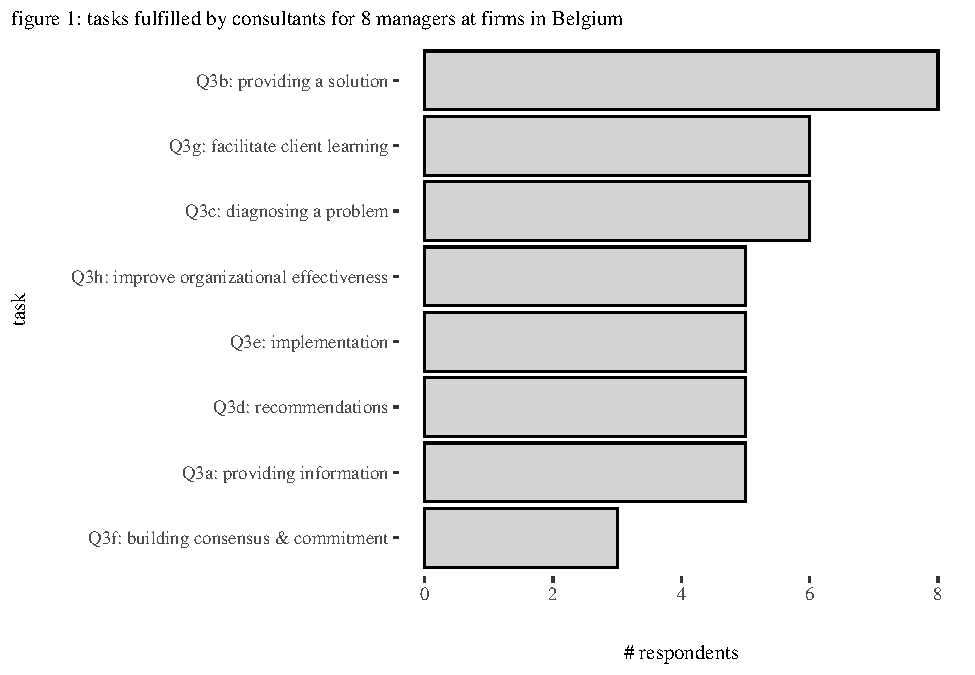
\includegraphics{2_ams_five_pager_files/figure-latex/unnamed-chunk-2-1.pdf}

\subsection{Rationale (RQ2)}\label{rationale-rq2}

There is a clear pattern when it comes to the rationale for hiring
consultants. They have the skills that are not available in-house, or
they are hard to recruit. Furthermore, they're the experts in the tasks
that they are hired for, and they can look at it with an outsider
perspective.

Respondent 3 explicitly mentioned that a consultant is their soundboard:
the respondent has the inside knowledge, and the consultants has
knowledge about the task at hand. A back-and-forth with a consultants is
an iteration to come to the best solution for the company. Respondent 1
agreed. Consultants are good at tasks with low asset specificity.
Without the necessary commitment, it's impossible to grasp the company.
Only employees, with long-term commitment, succeed at grasping the
complex product of the company.

Multiple respondents mentioned how hard it is today to hire people for
specific tasks, and for which they are forced to rely on consultants.
They claim that this is a Belgian problem: tech-savvy people are seduced
with a higher wage and fringe benefits that only consultancy firms can
offer. Furthermore, lots of senior experts become freelance consultants
due to its fiscally attractive regime.

The topic of cost control and/or cost reduction sparked discussion with
three respondents. For respondent 1, hiring consultants vis-à-vis
recruiting new staff meant an internalization of costs and that it was
added to the P\&L. Respondent 2 explained how consultants were often
chosen as it was easy to assess beforehand what the cost would be.
Finally, respondent 7 described how many managers preferred consultants
because they don't come with indirect costs like unionization \& pension
scheme obligations.

\(~\)

\begin{center}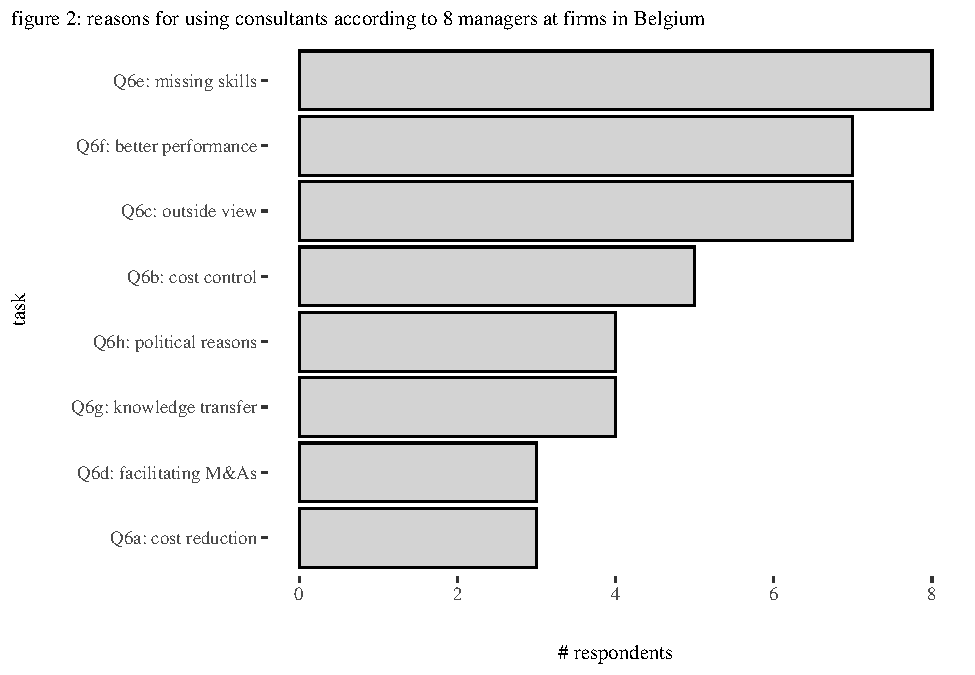
\includegraphics[width=0.75\linewidth]{2_ams_five_pager_files/figure-latex/unnamed-chunk-3-1} \end{center}

\subsection{Success (RQ3)}\label{success-rq3}

A clear picture emerged when asking the respondents about how they
define and evaluate the success of a consultancy engagement. Most
respondents have no formal, objective way for determining if a
consultancy engagement was successful. Respondent 1 described how there
are statements of work, but no statements of success. When problems
arise during a consultancy assignment, this results in a mutual blame
game. Respondent 5 admitted they never even considered what defines a
successful consultancy engagement.

Two informal definitions of success did, however, arise during the
follow-up discussion for this question. - The job is done. - The
respondent and the consultant hit it off.

The first is objective, yet almost tautological. Furthermore, it does
not account for any kinds of moral hazard that could have occurred
during the engagement. Finally, it does not take into account the
opportunity costs when a task could have been done internally.

The second is completely subjective, and hard to rationalize. This
hard-to-define bond between a manager and a consultants shows that
there's at least some truth in the more critical theoretical frameworks,
like social identity theory.

\subsection{Agency Problems (RQ4)}\label{agency-problems-rq4}

\subsection{Controlling Adverse Selection
(RQ5)}\label{controlling-adverse-selection-rq5}

\subsection{Controlling Moral Hazard
(RQ6)}\label{controlling-moral-hazard-rq6}

\section{Limitations}\label{limitations}

\section{Conclusions}\label{conclusions}

\bibliographystyle{apalike}
\renewcommand\refname{References}
\bibliography{references.bib}



\end{document}
